\documentclass[10pt,conference]{IEEEtran}
\IEEEoverridecommandlockouts

\usepackage{cite}
\usepackage{kotex}
\usepackage{float}
\usepackage{amsmath,amssymb,amsfonts}
\usepackage[ruled, vlined]{algorithm2e}
\usepackage{graphicx}
\usepackage{textcomp}
\usepackage{xcolor}
\usepackage{listings}
\usepackage{caption}
\usepackage{subcaption}
\usepackage{multirow}
\usepackage{booktabs}
\usepackage{makecell}

% load macros
% names
\newcommand{\cfg}{\text{CFG}}
\newcommand{\bnf}{\text{BNF}}
\newcommand{\es}{\text{ES}}
\newcommand{\bnfes}{\bnf_\es}
\newcommand{\peg}{\text{PEG}}

% codes
\newcommand{\scode}[1]{\texttt{\scriptsize#1}}
\newcommand{\code}[1]{\texttt{\footnotesize#1}}
\newcommand{\kwtrue}{\code{true}}
\newcommand{\kwt}{\code{\#t}}
\newcommand{\kwfalse}{\code{false}}
\newcommand{\kwf}{\code{\#f}}

%BNF_ES
\newcommand{\symb}{s}
\newcommand{\NT}[1]{#1}
\newcommand{\T}[1]{\code{#1}}
\newcommand{\argument}{a}
\newcommand{\param}{p}
\newcommand{\butnot}{\!\smallsetminus\!}
\newcommand{\rhs}{\alpha}
\newcommand{\cond}{c}
\newcommand{\nolt}{\left<\neg\code{LT}\right>}

% colors
\newcommand{\inred}[1]{{\color{red}{#1}}}

% lookahead
\newcommand{\symbfirst}[1]{\textbf{first}_\symb(#1)}
\newcommand{\rhsfirst}[1]{\textbf{first}_\rhs(#1)}
\newcommand{\fail}{FAIL}
\newcommand{\emptyfirst}{\circ}
\newcommand{\firstplus}{:\!\!+\;}
\newcommand{\la}{L}
\newcommand{\getlap}[1]{\textbf{get}_\symb(#1)}

% IR_ES language
\newcommand{\ires}{\text{IR}_\text{ES}}
\newcommand{\tend}{\downarrow}
\newcommand{\tin}{\searrow}
\newcommand{\tout}{\swarrow}
\newcommand{\tstar}{\star}

% hint image
\newcommand{\hint}{%
  \begingroup\normalfont
  \includegraphics[height=\fontcharht\font`\B]{img/hint.png}%
  \endgroup
}

% Our tool name
\newcommand{\tool}{\text{\sf JSECT}}
\newcommand{\jiset}{\text{\sf JISET}}

% K framework
\newcommand{\kframework}{\mathbb{K}}

% IRES
\newcommand{\irinst}{i}
\newcommand{\irexpr}{e}
\newcommand{\irvalue}{v}
\newcommand{\irstate}{\sigma}

% Scala code style
\definecolor{dkgreen}{rgb}{0,0.6,0}
\definecolor{gray}{rgb}{0.5,0.5,0.5}
\definecolor{mauve}{rgb}{0.58,0,0.82}
\lstdefinestyle{myScalastyle}{
  frame=tb,
  language=scala,
  aboveskip=3mm,
  belowskip=3mm,
  showstringspaces=false,
  columns=fixed,
  basicstyle={\footnotesize\ttfamily},
  numbers=none,
  keywordstyle=\color{blue},
  commentstyle=\color{dkgreen},
  stringstyle=\color{mauve},
  frame=single,
  breaklines=true,
  breakatwhitespace=true,
  tabsize=3,
}
\lstdefinestyle{smallScalastyle}{
  frame=tb,
  language=scala,
  aboveskip=3mm,
  belowskip=3mm,
  showstringspaces=false,
  columns=fixed,
  basicstyle={\scriptsize\ttfamily},
  numbers=none,
  keywordstyle=\color{blue},
  commentstyle=\color{dkgreen},
  stringstyle=\color{mauve},
  frame=single,
  breaklines=true,
  breakatwhitespace=true,
  tabsize=3,
}

% ECMAScript Intermediate Reprentations
\lstdefinestyle{ires}{
  frame=tb,
  aboveskip=3mm,
  belowskip=3mm,
  showstringspaces=false,
  columns=fixed,
  basicstyle={\footnotesize\ttfamily},
  numbers=none,
  keywordstyle=\color{blue},
  commentstyle=\color{dkgreen},
  stringstyle=\color{mauve},
  frame=single,
  breaklines=true,
  breakatwhitespace=true,
  tabsize=3,
}

% JavaScript code style
\lstdefinelanguage{JavaScript}{
  keywords={typeof, new, true, false, catch, function, return, null, catch, switch, var, if, in, while, do, else, case, break},
  keywordstyle=\color{blue}\bfseries,
  ndkeywords={class, export, boolean, throw, implements, import, this},
  ndkeywordstyle=\color{darkgray}\bfseries,
  identifierstyle=\color{black},
  sensitive=false,
  comment=[l]{//},
  morecomment=[s]{/*}{*/},
  commentstyle=\color{purple}\ttfamily,
  stringstyle=\color{red}\ttfamily,
  morestring=[b]',
  morestring=[b]"
}

\lstdefinestyle{myJSstyle}{
  language=JavaScript,
  extendedchars=true,
  basicstyle=\footnotesize\ttfamily,
  showstringspaces=false,
  showspaces=false,
  numbers=none,
  tabsize=2,
  breaklines=true,
  showtabs=false,
  captionpos=b
}


\begin{document}

\title{$\textsf{JEST}$: $N\!+\!1$-version Differential Testing of\\ Both JavaScript Engines and Specification}

% \title{$N\!+\!1$-differential Testing of Both JavaScript Engines and
% Specification via Mechanized Specification Extraction}

% \title{$\tool$: $N\!+\!1$-differential Testing of JavaScript}

% \title{Automated Generation of Conformance Tests for JavaScript Engines from ECMAScript}

% \title{$N\!+\!1$-differential Testing by Automatic Test Generation
% for JavaScript Engines and ECMAScript}

\author{
  \IEEEauthorblockN{Anonymous Author(s)}
}

% \author{
%   \IEEEauthorblockN{Jihyeok Park}
%   \IEEEauthorblockA{\textit{School of Computing} \\
%   \textit{KAIST}\\
%   Daejeon, South Korea\\
%   jhpark0223@kaist.ac.kr}
% 
%   \and
% 
%   \IEEEauthorblockN{Seungmin An}
%   \IEEEauthorblockA{\textit{School of Computing} \\
%   \textit{KAIST}\\
%   Daejeon, South Korea\\
%   h2oche@kaist.ac.kr}
% 
%   \and
% 
%   \IEEEauthorblockN{Dongjun Youn}
%   \IEEEauthorblockA{\textit{School of Computing} \\
%   \textit{KAIST}\\
%   Daejeon, South Korea\\
%   f52985@kaist.ac.kr}
% 
%   \and
% 
%   \IEEEauthorblockN{Gyeongwon Kim}
%   \IEEEauthorblockA{\textit{School of Computing} \\
%   \textit{KAIST}\\
%   Daejeon, South Korea\\
%   gyeongwon.kim@kaist.ac.kr}
% 
%   \and
% 
%   \IEEEauthorblockN{Sukyoung Ryu}
%   \IEEEauthorblockA{\textit{School of Computing} \\
%   \textit{KAIST}\\
%   Daejeon, South Korea\\
%   sryu.cs@kaist.ac.kr}
% }

\maketitle

\begin{abstract}
  Modern programming follows the continuous integration (CI) and continuous
  deployment (CD) approach rather than the traditional waterfall model.  Even
  the development of modern programming languages uses the CI/CD approach to
  swiftly provide new language features and to adapt new development
  environments.  Unlike the conventional approaches, in the modern CI/CD
  approaches, the language specification is no more the Oracle of semantics
  because both the specification and interpreters (or compilers) can co-evolve.
  In this setting, both the specification and implementations may have bugs, and
  guaranteeing their correctness is non-trivial.

  In this paper, we present a novel \textit{$N$+1-version testing} to resolve
  the problem.  Unlike the traditional $N$-version testing, our approach
  consists of three steps: 1) to automatically synthesize programs guided by the
  syntax and semantics from the given language specification, 2) to generate
  conformance tests by injecting assertions to them to check their final program
  states, and 3) to find and localize the specification bugs via executing
  programs on multiple implementations.  We propose \( \tool \) that performs
  $N$+1-version testing for modern JavaScript engines and ECMAScript, which is
  the specification of JavaScript that describes syntax and semantics in a
  natural language.  We evaluated our tool with four JavaScript engines that
  support all modern JavaScript language features and the most recent version of
  ECMAScript (ES11, 2020).  \( \tool \) automatically synthesized \inred{X,XXX}
  programs that covered \inred{XX.XX\%} of syntax and \inred{XX.XX\%} of
  semantics from ES11.  Using the assertion-injected JavaScript programs, our
  tool found \inred{XX} engine bugs in four different engines and \inred{X}
  specification bugs in ES11.
\end{abstract}


\begin{IEEEkeywords}
JavaScript, conformance test generation, mechanized specification,
differential testing
\end{IEEEkeywords}

\section{Introduction}\label{sec:intro}

In Peter O'Hearn's keynote speech in ICSE 2020, he quoted the following from
Mark Zuckerberg's Letter to Investors~\cite{mzletter}:
\begin{quote}
  The Hacker Way is an approach to building that involves continuous improvement
  and iteration.  Hackers believe that somethings can always be better, and that
  nothing is ever complete.
\end{quote}
Indeed, modern programming follows the continuous integration (CI) and
continuous deployment (CD) approach~\cite{cicd} rather than the traditional waterfall model.
Instead of a sequential model that divides software development into
several phases, each of which takes time, CI/CD amounts to a cycle of
quick software development, deployment, and back to development with
feedback. Even the development of programming languages uses the CI/CD approach.

Consider JavaScript, which is one of the most widely used programming languages
not only for client-side but also for server-side programming~\cite{nodejs} and
even for embedded systems~\cite{moddable,espruino,tessel2}.  Various JavaScript
engines provide diverse extensions to adapt to fast-changing user demands.  At
the same time, ECMAScript, the official specification that describes the syntax and
semantics of JavaScript, is annually updated since ECMAScript 6 (ES6,
2015)~\cite{es6} to support new language features in response to user demands.
Such updates in both the specification and implementations in tandem make it
difficult for them to be in sync.

Another example is Solidity~\cite{officialSolDoc}, the standard smart contract programming language
for the Ethereum blockchain.  The Solidity language specification is continuously
updated, and the Solidity compiler is also frequently released.  According to
Hwang and Ryu~\cite{solidity-gap}, the average number of days between consecutive
releases from Solidity 0.1.2 to 0.5.7 is 27.  In most cases, the Solidity compiler reflects
updates in the specification, but even the specification is revised
according to the semantics implemented in the compiler.  As in JavaScript,
bidirectional effects in the specification and the implementation make
it hard to guarantee their correspondence.

The conventional approach to build a programming language is uni-directional from
a language specification to its implementation.  The specification is believed to
be correct and the conformance of an implementation to the specification is
checked by dynamic testing.  Unlike in the conventional approach, in the modern CI/CD
approach, the specification may not be the Oracle, because both the
specification and the implementation can co-evolve.  In this setting, both the
specification and the implementation may contain bugs, and guaranteeing their
correctness is a challenging task.

In this paper, we propose a novel \textit{$N$+1-differential testing}, which
enables testing of co-evolving specifications and their implementations.  The
differential testing~\cite{diff-test} is a testing technique, which executes $N$
implementations of a specification concurrently for each input, and detects a
problem when the outputs are in disagreement.  In addition to $N$
implementations, our approach tests the specification as well using the
mechanized specification.  Recently, several approaches to extract syntax and
semantics directly from language specifications are presented\cite{jiset,
extract-x86, extract-arm}.  We utilize them to bridge the gap between
specifications and their implementations through conformance tests generated
from mechanized specifications.  The $N$+1-differential testing consists of
three steps: 1) to automatically synthesize programs guided by the syntax and
semantics from a given language specification, 2) to generate conformance tests
by injecting assertions to the synthesized programs to check their final program
states, and 3) to find and localize bugs in the specification and
implementations via executing the conformance tests on multiple implementations.

Given a language specification and $N$ existing real-world
implementations of the specification, we
automatically generate a conformance test suite from the specification with
assertions in each test code to make sure that the result of running the code
conforms to the specification semantics.  Then, we run the test suite for $N$
implementations of the specification.  Because generated tests strictly comply
with the specification, they reflect specification errors as well, if any.  When
one of the implementations fails in running a test, it is highly likely that the
implementation has a bug, which is the traditional differential testing.  When
most of the implementations fail in running a test, it is highly likely that
the specification has a bug.  By automatically generating a rich set of test
code from the specification and running them with implementations of the
specification, we can find and localize bugs either in the specification written
in a natural language or in its implementations.

To show the practicality of the proposed approach, we present $\tool$, which
performs $N$+1-differential testing for modern JavaScript engines and ECMAScript.
We implement $\tool$ by extending $\jiset$~\cite{jiset}, which is a JavaScript
IR-based semantics extraction toolchain, to utilize syntax and semantics
automatically extracted from a given ECMAScript.  Using the extracted syntax,
our tool automatically synthesizes initial seed programs and expands the program
pool by mutating specific target programs guided by semantics coverage.  Then,
the tool generates conformance tests by injecting assertions to synthesized
JavaScript programs.  Finally, $\tool$ detects and localizes bugs via execution
results of the tests on $N$ JavaScript engines.  We evaluate our tool with four
JavaScript engines (GraalJS\cite{graaljs}, QuickJS\cite{qjs}, Moddable
XS\cite{xs}, and Google V8\cite{v8}) that support all modern JavaScript language
features and the most recent version of ECMAScript (ES11, 2020).

Our main contributions are as follows:
\begin{itemize}
  \item Present \textit{$N$+1-differential testing}, a novel solution to the new
    problem of the co-evolving language specification and implementation.
  \item Implement our solution in a tool $\tool$ for JavaScript engines with
    ECMAScript.  It is the first tool that automatically generates conformance
    tests for JavaScript engines from ECMAScript.  We first measure the coverage
    of Test262, the official conformance tests, as \inred{-}\% for statements
    and \inred{-}\% for branches.  The conformance tests generated by our tool
    has the coverage \inred{-}\% for statements and \inred{-}\% for branches.
  \item Evaluate $\tool$ with four modern JavaScript engines and the most recent
    version of ECMAScript, ES11.  Using the generated conformance test
    suite, our tool found and localized \inred{XX} engine bugs in four different
    engines and \inred{X} specification bugs in ES11.
\end{itemize}

\section{$N$+1-version Testing}\label{sec:idea}

In this section, we introduce the core concept of $N$+1-version testing with a
simple running example.  Then, we explain its overall structure consists of two
phases: a conformance test generation phase and a bug detection/localization
phase

\subsection{Main Idea}

The traditional $N$-version testing (or differential testing) utilizes the
cross-referencing Oracle, which is an assumption that any discrepency between
any program behaviors on the same input might be a potential bug.  Thus, it
compares the execution results of same inputs on different $N$ implementations
having same functionalities.  When an implementation provides a minority result
for a given input, it reports the implementation has a potential bug with the
input.

However, the $N$+1-version testing utilizes not only cross-referencing Oracle
from multiple implementations but also a mechanized specification.  It first
assumes that a mechanized specification as the Oracle and generates tests from
the specification.  Using the generated tests, it tests $N$ different
implementations and detects bugs.  Moreover, if most of implementations fail to
pass a test for the same reason, we are doubtful of the existence of bugs in
the specification.  Thus, $N$+1-version testing assumes that there exists a
specification bugs related to the test in this situation and localizes the bugs
in the specification based on the statistical information.


\subsection{Running Example}

\begin{figure}[t]
  \centering
  \begin{subfigure}[t]{0.48\textwidth}
    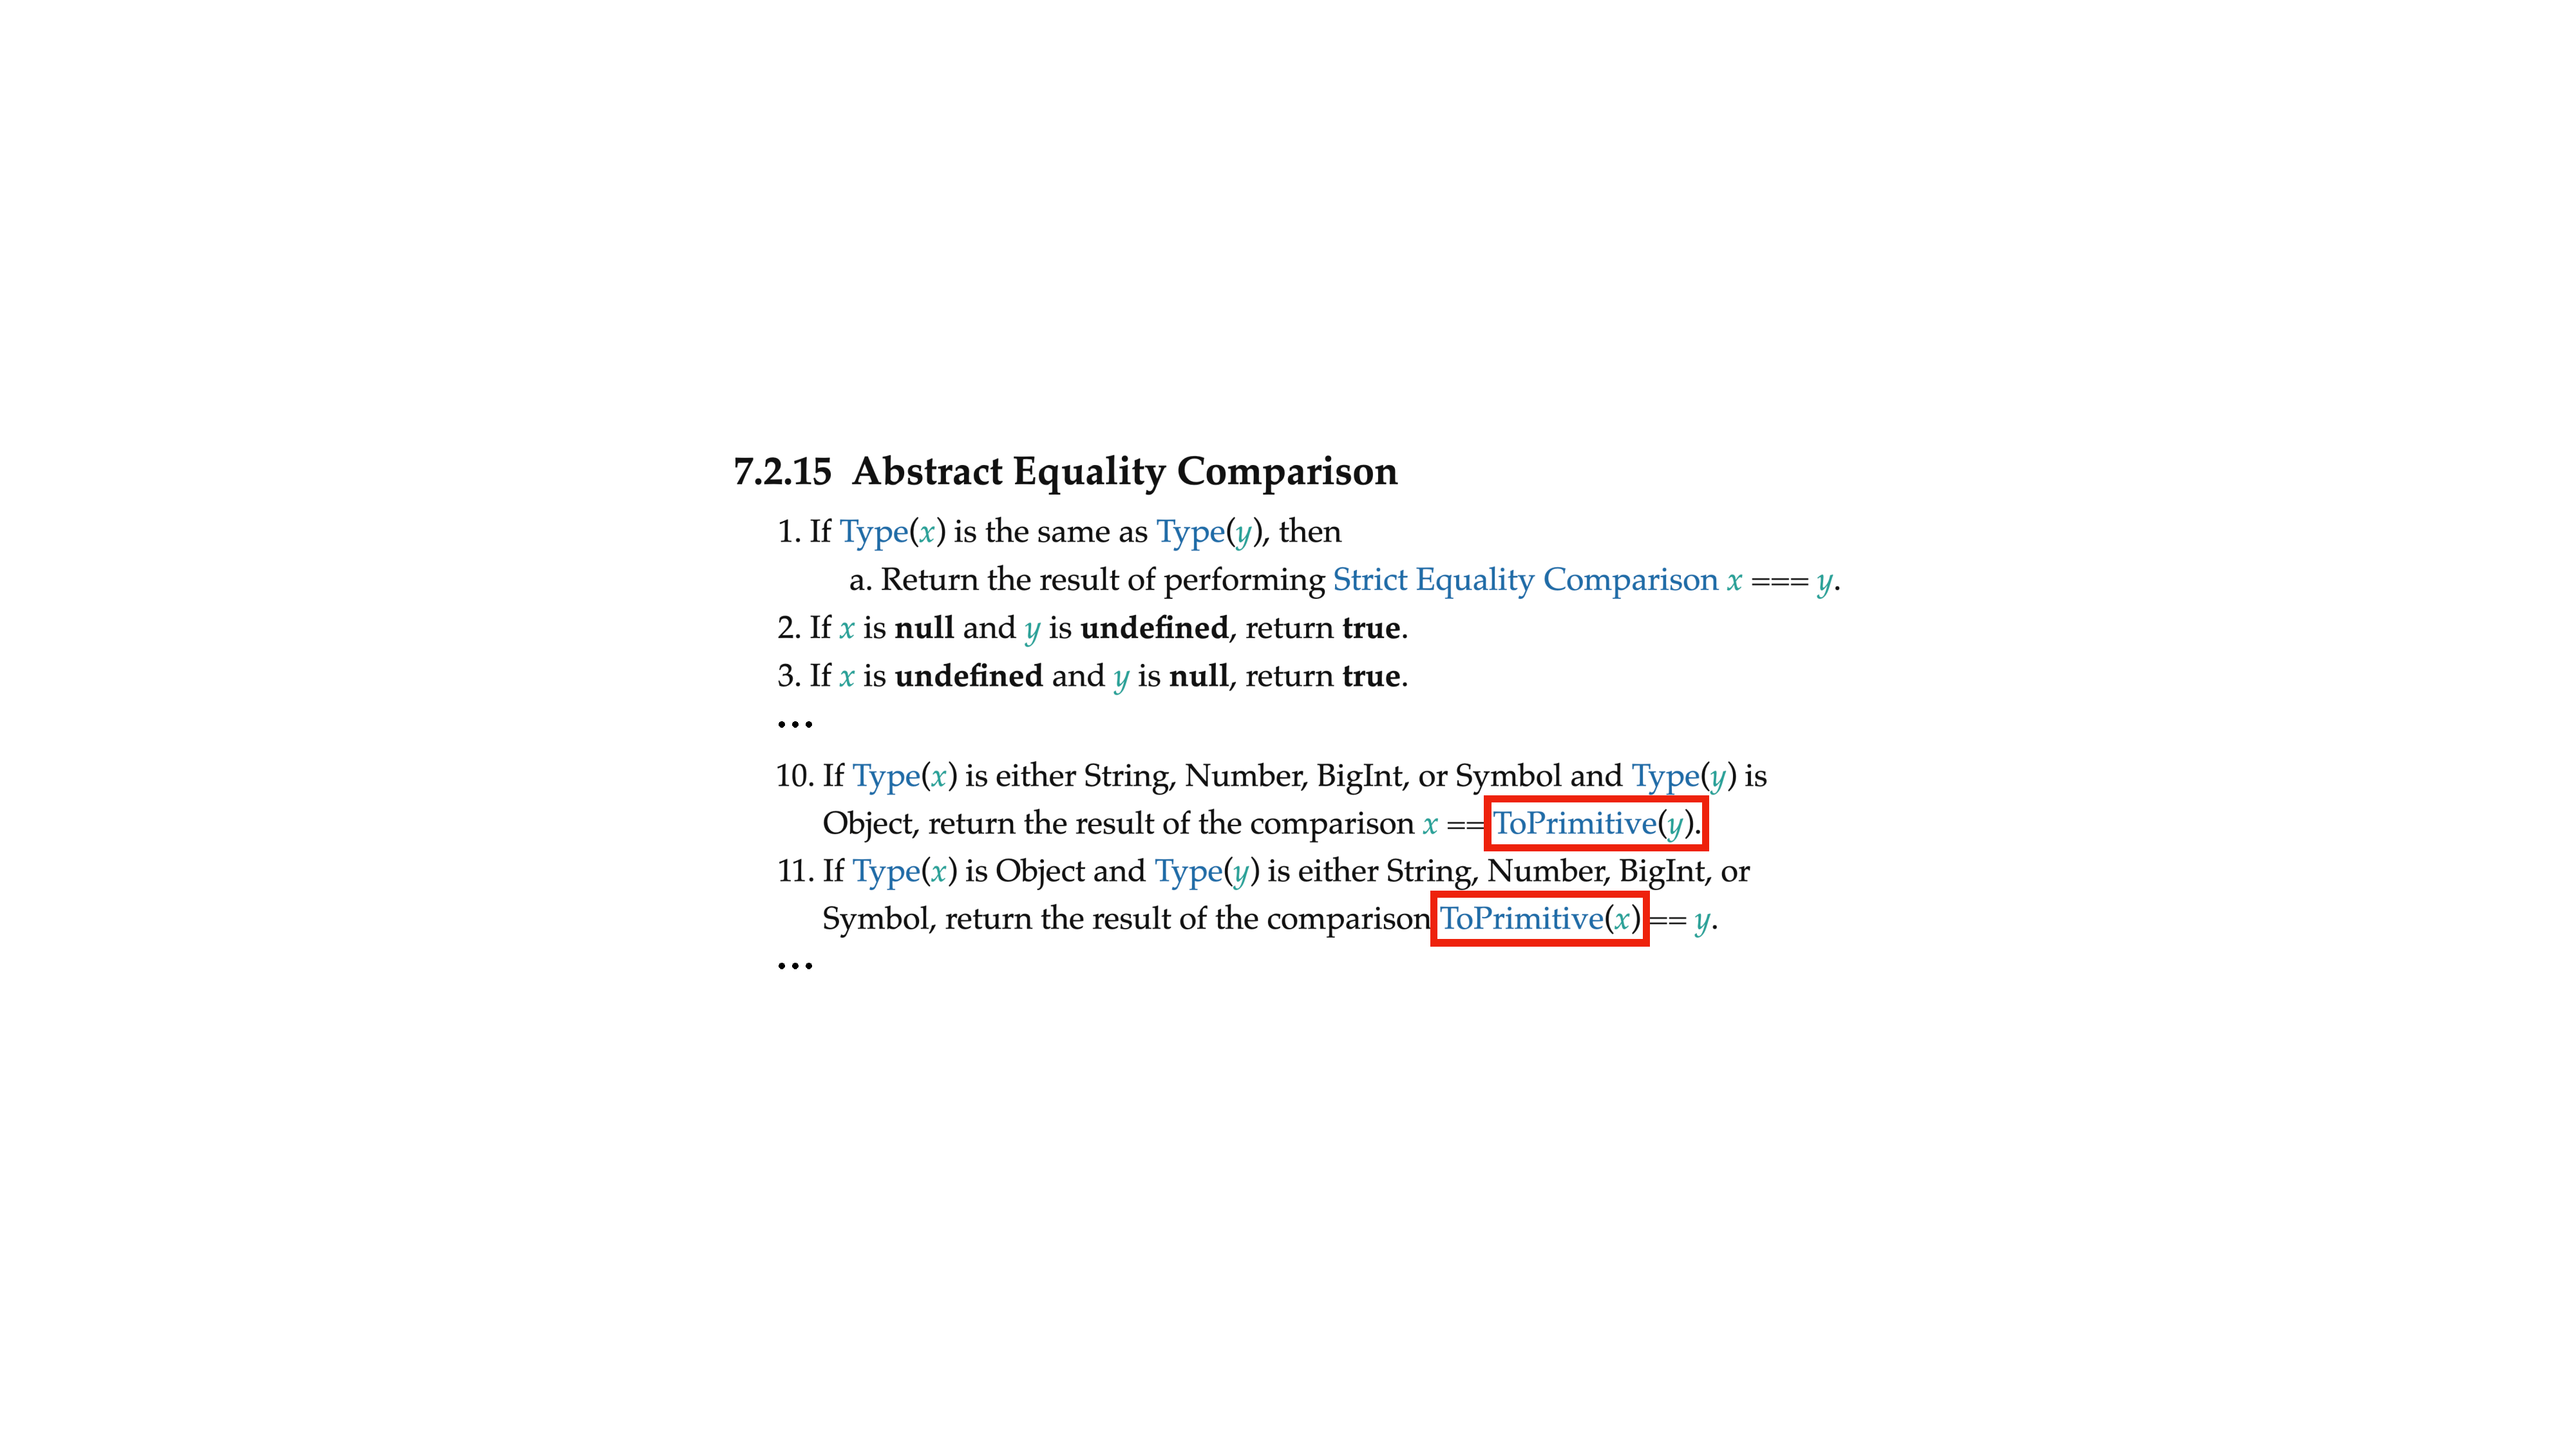
\includegraphics[width=\textwidth]{img/example-algo.pdf}
    \caption{The \textbf{Abstract Equality Comparison} abstract algorithm in
    ECMAScript 2020 (ES11)}
    \label{fig:example-algo}
  \end{subfigure}
  \begin{subfigure}[t]{0.43\textwidth}
    \begin{lstlisting}[style=myJSstyle]
var obj = { valueOf: () => { throw 'err'; } };
var result = 42 == obj;
// expected: throw an exception with 'err'
// ES11 semantics: result === false
    \end{lstlisting}
    \caption{An example JavaScript program}
    \label{fig:example-js}
  \end{subfigure}
  \begin{subfigure}[t]{0.45\textwidth}
    \begin{lstlisting}[style=myJSstyle]
try {
  var obj = { valueOf: () => { throw 'err'; } };
  var result = 42 == obj;
  assert(result === false);
} catch (e) {
  assert(false);
}
    \end{lstlisting}
    \caption{The assertion-injected JavaScript program}
    \label{fig:example-injected}
  \end{subfigure}
  \caption{A running example of $N$+1-version testing for JavaScript}
  \label{fig:example}
  \vspace*{-1em}
\end{figure}

\begin{figure*}[t]
  \centering
  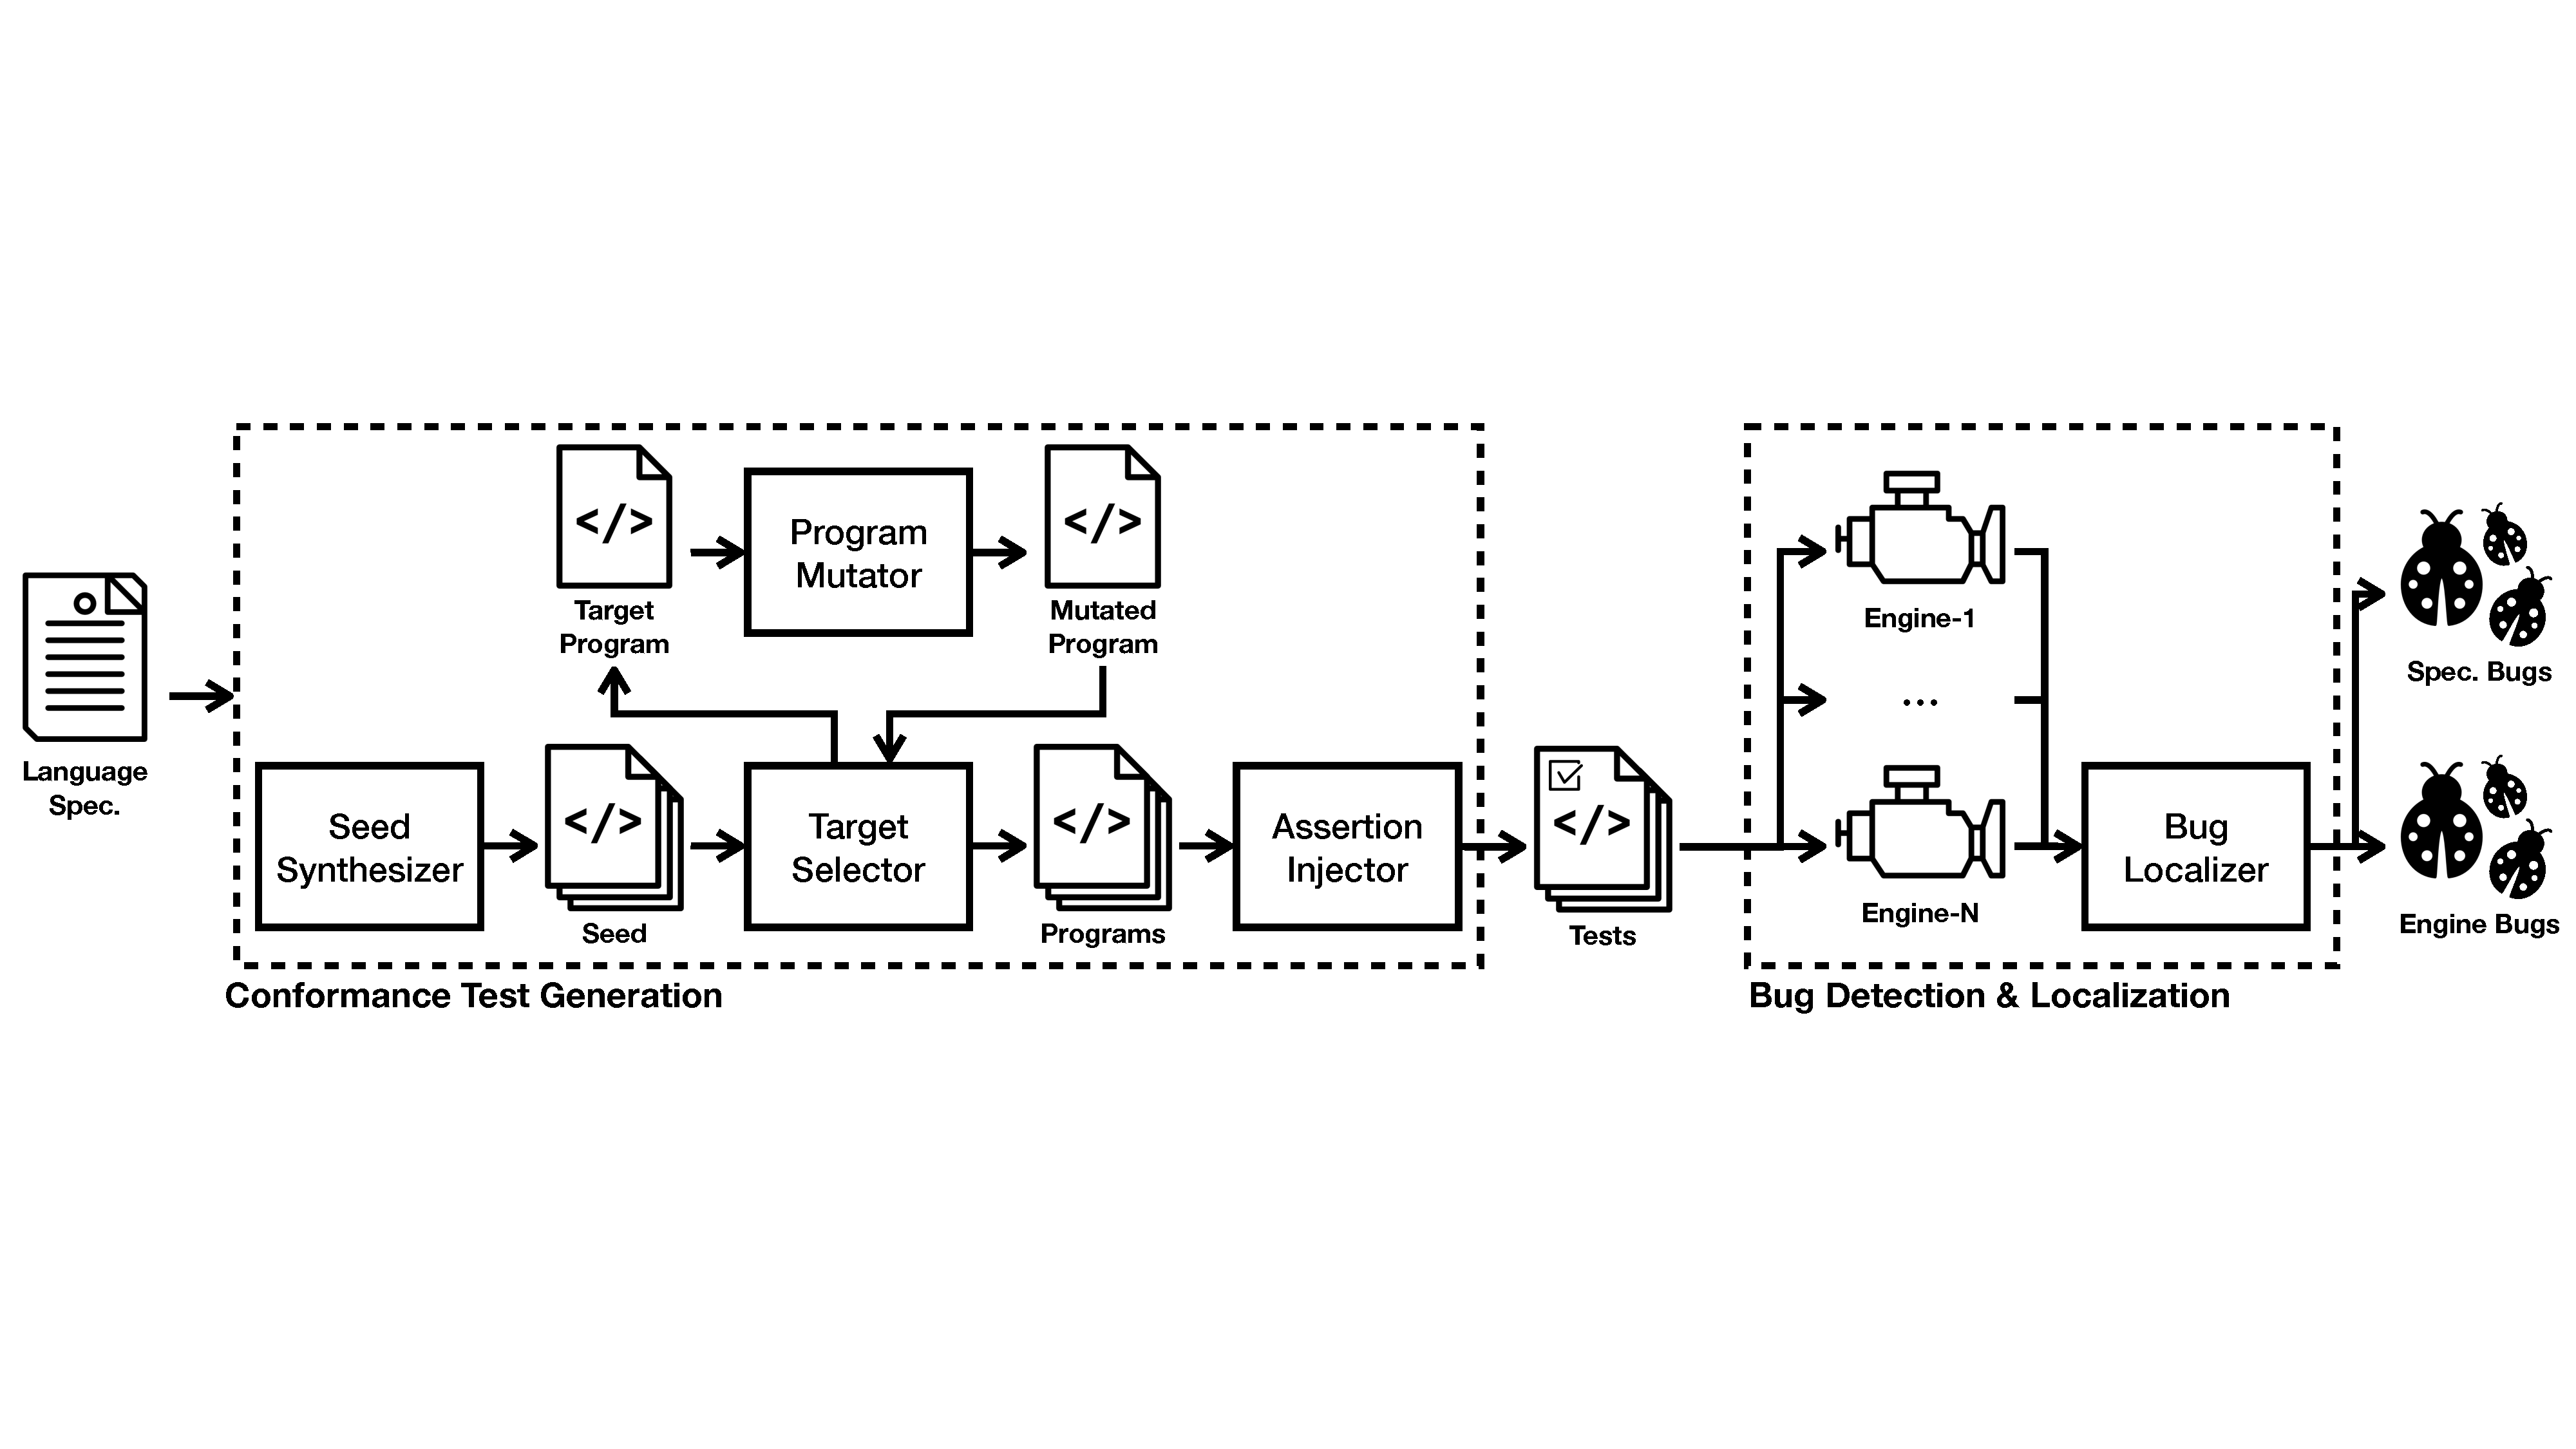
\includegraphics[width=0.95\textwidth]{img/n+1-version-testing.pdf}
  \caption{Overall structure of $N$+1-version testing for $N$ different
    implementations (engines) and a language specification.}
  \label{fig:overall}
  \vspace*{-1em}
\end{figure*}

Figure~\ref{fig:example} shows the running example of $N$+1-version for
JavaScript.  Figure~\ref{fig:example-algo} is a part of \textbf{Abstract Equality
Comparison} abstract algorithm in ECMAScript 2020 (ES11).  It describes the
semantics of non-strict equality comparison ($\code{==}$) between two JavaScript
values.  For example, $\code{null == undefined}$ is $\code{true}$ because of the
algorithm step 2.  According to step 10 and11, if a value has a String, Number,
BigInt, or Symbol type and the other value is an Object, the algorithm call the
\textbf{ToPrimitive} algorithm to convert the JavaScript object into a primitive
value and recursively call itself.  However, \textbf{ToPrimitive} algorithm
could return \textit{abrupt completion}.  ECMAScript uses completion values to
explain the runtime propagation of values and control flow such as behavior of
exceptions or $\code{break}$ statements.  When the type of a completion is not
$\code{normal}$ but one of $\code{break}$, $\code{continue}$, $\code{return}$,
and $\code{throw}$, the completion is called as an abrupt completion.  To handle
such abrupt completions, ECMAScript uses the question mark prefix (?) to check
and pass out the abrupt completions.  However, invocations of
\textbf{ToPrimitive} in step 10 and 11 do not use the question mark prefix (?).
Thus, it cannot pass out the exceptions introduced by \textbf{ToPrimitive} to
outisde.

For example, the JavaScript code in Figure~\ref{fig:example-js} causes the above
problem.  In the \textbf{Abstract Equality Comparison} algorithm, variables
\textit{x} and \textit{y} denote $\code{42}$ and an object whose property
$\code{valueOf}$ points to an arrow function that throws an error.  In step 10,
the object is passed to the \textbf{ToPrimitive} function and it returns an
abrupt completion because the function stored in $\code{valueOf}$ throws an
error.  However, the specification silently ignores the abrupt completion and
returns $\code{false}$ as the result of comparison.  Based on the semantics
described in the specification, we could inject assertions to check the code
does not throw any erros as described in Figure~\ref{fig:example-injected}.
However, most of modern JavaScript engines throw an error with a string
$\code{'err'}$.  Using this information, we know that there exists a potential
specification bug with the JavaScript code.  Moreover, we can localize the
detected bug using the statistical information. Among bunch of conformance
tests, most of tests that go through steps 10 and 11 in the algorithm would be
fail in most of JavaScript engines.  It gives us the information that the bug
exists in the steps 10 and 11 of \textbf{Abstract Equality Comparison} with high
probability.


\subsection{Overall Structure}

Figure~\ref{fig:overall} depicts the overall structure of $N$+1-verison testing
for $N$ different engines and a language specification.  It consists of two
phases: a conformance test generation phase and a bug detection/localization
phase.  Based on a given language specification, it automatically generates
conformance tests that reflect the language syntax and semantics described in
the specification.  Then, it detects and localizes engine or specification bugs
via results of the generated tests on $N$ different engines.  Now, we introduce
each module in $N$+1-version testing and explain its functionalities.
\newline

\subsubsection{Seed Synthesizer}
At the first step, \textsf{Seed Synthesizer} synthesizes initial seed programs
based on the language syntax.  Its main goal is to synthesize 1) few number of
2) small sized programs 3) that cover possible cases in syntax rules as many as
possible.
\newline

\subsubsection{Target Selector}
For a given program pool, it selects a target program in the program pool
depending on the semantics coverage of program pool.  The initial program pool
is the seed programs generated by \textsf{Seed Synthesizer}. The program pool
will be grown by adding a new program mutated by \textsf{Program Mutator} from
the selected target program.  When specific criteria are satisfied,
\textsf{Target Selector} stops to select target program and gives programs in
the current program pool as the result.
\newline

\subsubsection{Program Mutator}
The main goal of \textsf{Program Mutator} is to generate a new program my
mutating a given target program in order to increase the semantics coverage.
If it fails to generate a new program to increase semantics coverage,
\textsf{Target Selector} selects a new target program again and repeat this
process less than the pre-defined maximum trial number.
\newline

\subsubsection{Assertion Injector}
It modifies given programs to conformance tests by injecting appropriate
assertions reflecting the semantics described in the specification.
\textsf{Assertion Injector} executes each program under the mechanized
specification and obtains the final state of the execution.  Based on the final
state, it automatically inject assertions to the program.
\newline

\subsubsection{Bug Localizer}
First, it executes the given conformance tests on $N$ different engines and
collects the test results.  For each test, if minor engines fail,
it reports the potential bugs in the engines fail the test.  Otherwise, it
reports the potential bugs in the specification.  It utilizes \textit{coverage
based statistical fault localization} (CBSFL)~\cite{fault-local}.  It uses coverage
information of tests to rank the statements from most suspicious to least
suspicious ones.

% 참고 https://hackthology.com/how-to-evaluate-statistical-fault-localization.html

\section{Application: JavaScript}\label{sec:application}

We actualize $N$+1-version testing approach for the JavaScript programming
language via $\tool$, that utilizes modaern JavaScript engines and ECMAScript.
It extends $\jiset$ to automatically construct sub-modules for $N$+1-version
testing.  In this section, we explain each module consisting $\tool$ in detail.

\subsection{Seed Synthesizer}

To synthesize seed JavaScript programs, we implement two different
synthesizers: \textit{non-recursive synthesizer} and \textit{built-in function
synthesizer}.
\newline

\subsubsection{Non-Recursive Synthesizer}

The main goal of the non-recursive synthesizer is to cover various cases of
syntax.  It consists of two steps: 1) to find the shortest string for each
non-terminal and 2) to synthesize JavaScript programs using the pre-calculated
shortest strings.  While we support various extended rules in grammar of
ECMAScript such as parametric non-terminals, conditional alternatives, and
various special terminal symbols, we focus on simple terminals and non-terminals
in this section for the brevity.

\begin{algorithm}[t]
  \caption{Worklist-based Shortest String}
  \label{alg:short-string}
  \DontPrintSemicolon
  \SetKwProg{Fn}{Function}{:}{}
  \SetKwFunction{shortestStrings}{shortestStrings}
  \SetKwFunction{update}{update}
  \SetKwFunction{propagate}{propagate}
  \KwIn{$\ruleset$ - syntax reduction rules}
  \KwOut{$M$ - map from non-terminals to shortest strings}
  \Fn{\shortestStrings{$\ruleset$}} {
    $M = \varnothing, \worklist = \text{a queue that consists of}\ \ruleset$\;
    \While{$\worklist \neq \varnothing$} {
      $\text{pop}\ (A, \alpha) \gets \worklist$\;
      \lIf{$\update(A, \alpha)$} {
        $\propagate(\worklist, \ruleset, A)$
      }
    }
  }
  \Fn{\update{$A, \alpha$}} {
    $str = \text{an empty string}$\;
    \ForAll{$s \in \alpha$} {
      \lIf{$s\ \text{is a terminal}\ t$} {
        $str = str + t$
      }
      \ElseIf{$s\ \text{is a non-terminal}\ A \wedge A \in M$} {
        $str = str + M[A]$
      }
      \lElse {
        \Return false
      }
    }
    \lIf{$\exists M[A] \wedge \norm{str} \geq \norm{M[A]}$} {
      \Return false
    }
    $M[A] = str$\;
    \Return true\;
  }
  \Fn{\propagate{$\worklist, \ruleset, A$}} {
    \ForAll{$(A', \alpha') \in \ruleset$} {
      \lIf{$A \in \alpha'$} {
        $\text{push}\ (A', \alpha') \rightarrow \worklist$
      }
    }
  }
\end{algorithm}

For the first step, we find the shortest string for each non-terminal via the
\textsf{shortestStrings} function described in Algorithm~\ref{alg:short-string}.
We modifies the algorithm introduced by McKenize~\cite{cfg-gen} to find the
shortest string instead of a random string.  It takes syntax reduction rules
$\ruleset$, which is a set of pairs of non-terminals and alternatives and
returns a map $M$ from non-terminals to their shortest strings.  It utilizes a
worklist $W$, which is a queue structure that includes syntax reduction rules
that affected by updated non-terminals.  The function initializes the worklist
$W$ with all syntax reduction rules $\ruleset$.  Then, it extracts a syntax
reduction rule $(A, \alpha)$, updates the map $M$ via the \textsf{update}
function, and propagate updated information via the \textsf{propagate} function.
The \textsf{update} function checks whether the given alternative $\alpha$ of
the non-terminal $A$ can derive a string shorter than the current shortest one
based on the current map $M$.  If it is possible, it stores the pair the
non-terminal $A$ and the newly found shortest string in the map $M$ and invokes
the \textsf{propagate} function.  The \textsf{propagate} function finds all
syntax reduction rules whose alternatives contains the updated non-terminal $A$
and inserts them into the worklist $W$.  The \textsf{shortestStrings} function
repeats this process until the worklist $W$ becomes empty.

\begin{algorithm}[t]
  \caption{Non-Recursive Synthesize}
  \label{alg:non-rec-synthesize}
  \DontPrintSemicolon
  \SetKwProg{Fn}{Function}{:}{}
  \SetKwFunction{nonRecSynthesize}{nonRecSynthesize}
  \SetKwFunction{getProd}{getProd}
  \SetKwFunction{getAlt}{getAlt}
  \KwIn{$\ruleset$ - syntax reduction rules, $S$ - start symbol}
  \KwOut{$D$ - set of strings derivable from $S$}
  \SetKwBlock{Begin}{function}{end function}
  \Fn{\nonRecSynthesize{$\ruleset, S$}} {
    $V = \varnothing, M = \shortestStrings(\ruleset)$\;
    \Return $\getProd(M, V, \ruleset, S)$\;
  }
  \Fn{\getProd{$M, V, \ruleset, A$}} {
    \lIf{$A \in V$} {
      \Return $\{ M[A] \}$
    }
    $D = \varnothing, V = V \cup \{ A \}$\;
    \ForAll{$(A', \alpha) \in \ruleset\ \text{s.t.}\ A' = A$} {
      $D = D \cup \getAlt(M, V, \ruleset, A, \alpha)$\;
    }
    \Return $D$\;
  }
  \Fn{\getAlt{$M, V, \ruleset, A, \alpha$}} {
    $L = \text{an empty list}$\;
    \ForAll{$s \in \alpha$} {
      \If{$s\ \text{is a terminal}\ t$} {
        $\text{append}\ (\{ t \}, t) \rightarrow L$\;
      }
      \ElseIf{$s\ \text{is a non-terminal}\ A'$} {
        $\text{append}\ (\getProd(M, V, \ruleset, A'), M[A])
        \rightarrow L$\;
      }
    }
    $D =$ point-wise concatenation of first elements of pairs in $L$ and use
    second elements for short cases.\;
    \Return $D$\;
  }
\end{algorithm}

After finding shortest strings for non-terminals, we synthesize programs via the
\textsf{nonRecSynthesize} function.  It takes syntax reduction rules $\ruleset$
and a start symbol $S$.  To reduce the number of redundant syntax elements, it
keeps the visited set $V$ of non-terminals and utilizes the map $M$ produced by
the \textsf{shortestStrings} function.  For the first visit with a non-terminal
$A$, The \textsf{getProd} function takes and returns unions of sets of strings
generated by invoking the \textsf{getAlt} algorithm with alternatives of the
non-terminal $A$.  However, if the already visited non-terminal $A$ is passed,
it returns the single shortest string $M[A]$.  The \textsf{getAlt} takes a
non-terminal $A$ with an alternative $\alpha$ and returns a set of strings
derivable from $\alpha$ via point-wise concatenation of strings derived by
symbols of $\alpha$.  If the numbers of strings derived by symbols are
different, the shortest strings are used to fill out the short cases.

\begin{figure}[t]
  \centering
  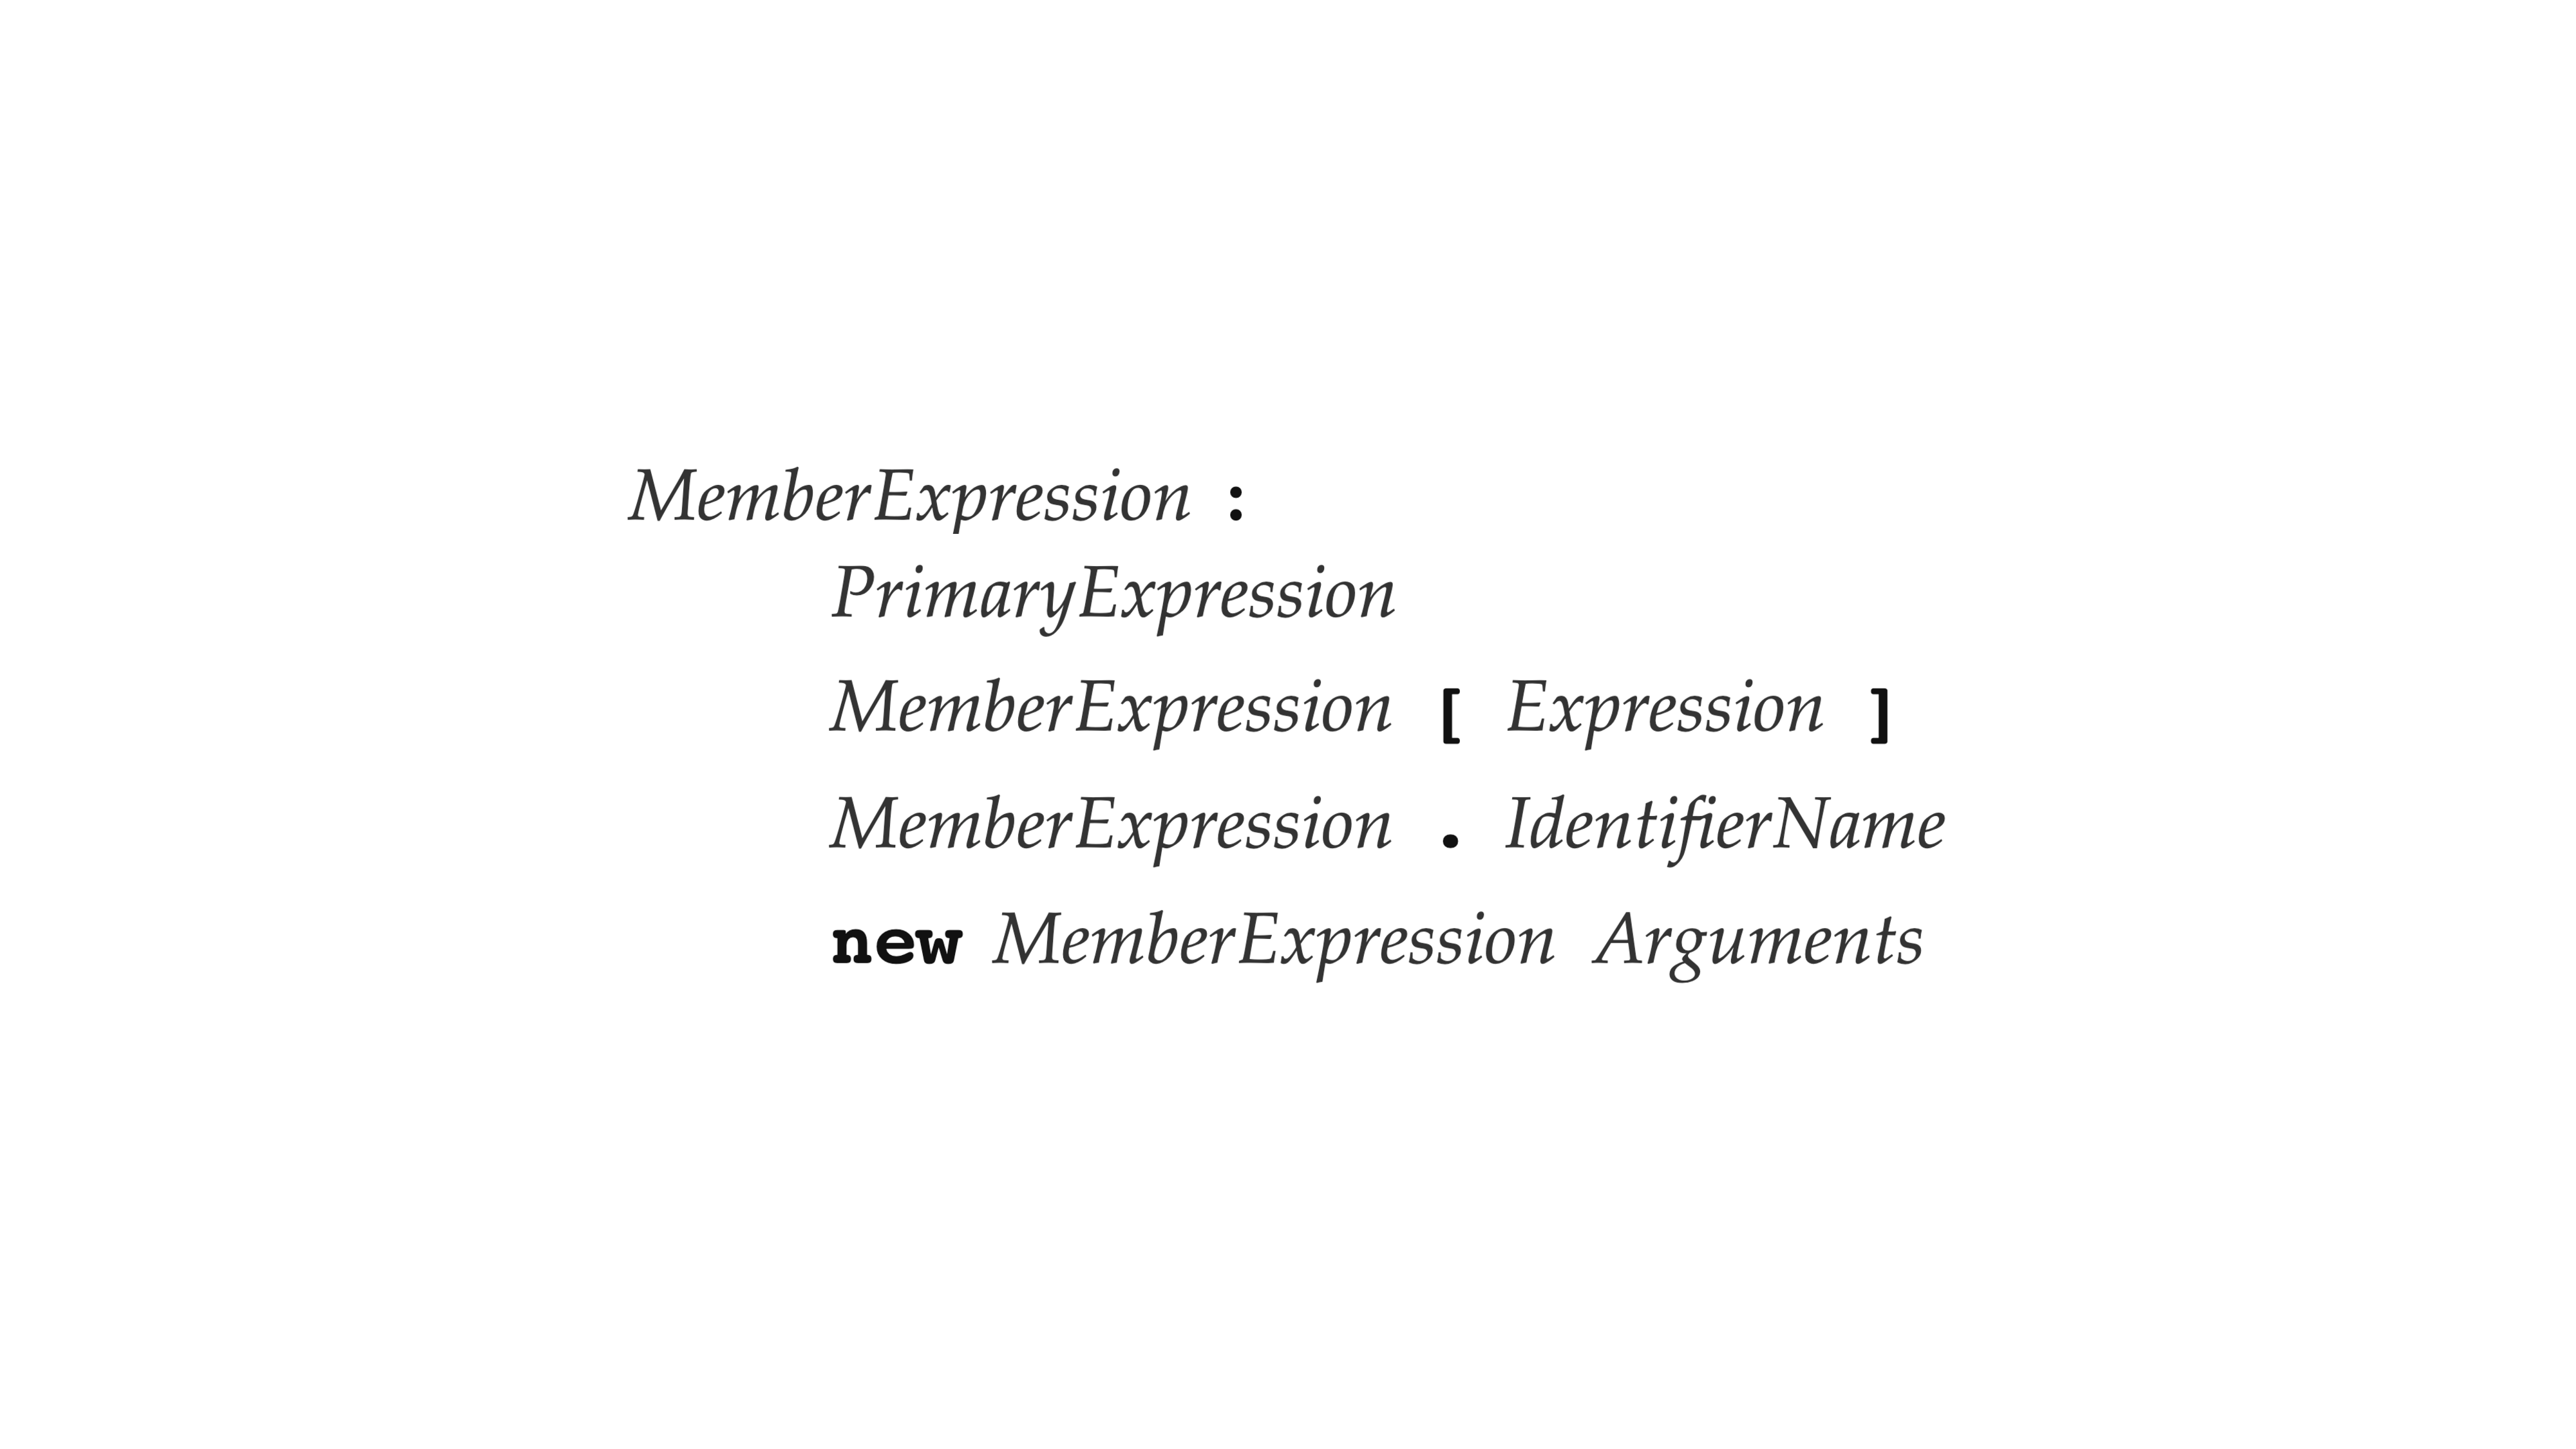
\includegraphics[width=0.32\textwidth]{img/syntax-member.pdf}
  \caption{The \textit{MemberExpression} production in ES11}
  \label{fig:prod-example}
  \vspace*{-1em}
\end{figure}

For example, Figure~\ref{fig:prod-example} shows the simplified
\textit{MemberExpression} production in ES11.  For the first step, we find
the shortest string for each non-terminal: \code{()} for \textit{Arguments} and
\code{x} for other non-terminals.  In the next step, we synthesize the strings
derivable from \textit{MemberExpression}.  The first alternative consists of a
single non-terminal \textit{PrimaryExpression} and it is the first time to visit
it.  Thus, it generates all cases of \textit{PrimaryExpression}.  The fourth
alternative consists of one terminal \code{new} and two non-terminals
\textit{MemberExpression} and \textit{Arguments}.  The \textit{MemberExpression}
is already visited thus it generates a single shortest string \code{x} but it is
the first time to visit \textit{Arguments}.  It generates all cases: \code{()},
\code{(x)}, \code{(...x)}, and \code{(x,)}.  However, the numbers of strings for
its symbols are different with each other.  To match the number of strings, we
fill out the short cases with terminal itself for \code{new} and the shortest
string \code{x} for \textit{MemberExpression} as follows:

\begin{figure}[H]
  \centering
  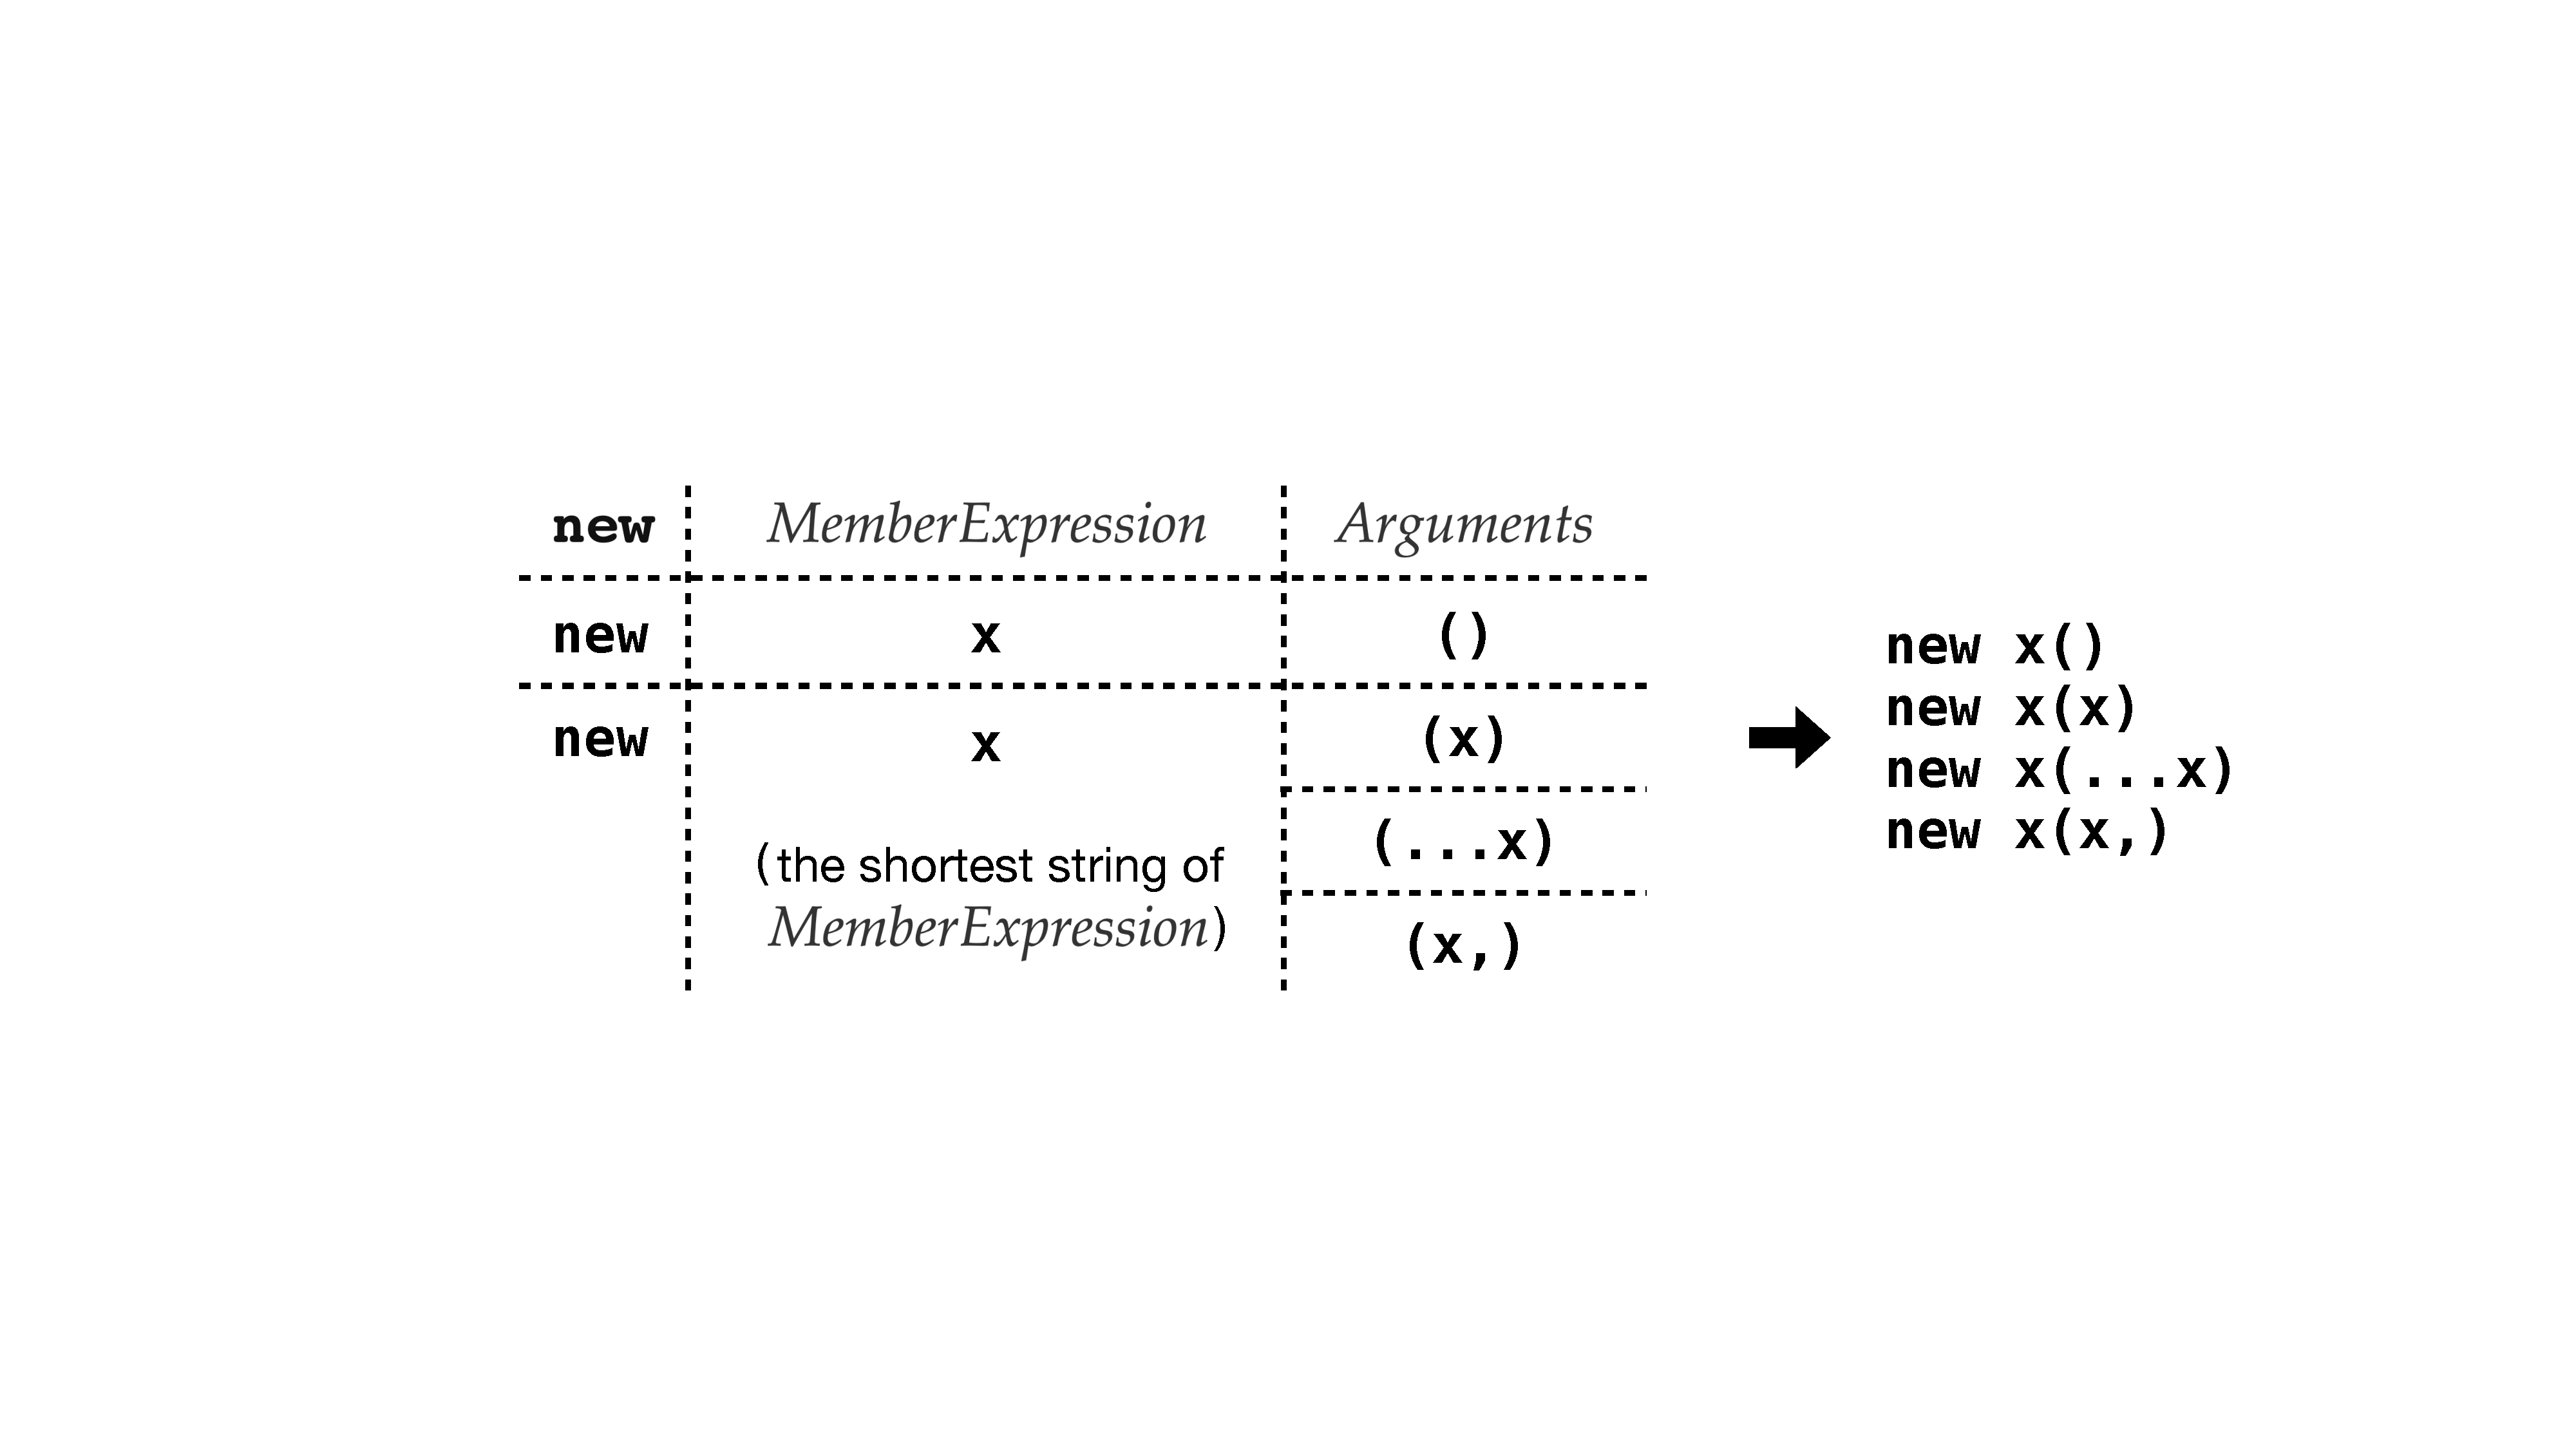
\includegraphics[width=0.48\textwidth]{img/member-example.pdf}
\end{figure}


\subsubsection{Built-in Function Synthesizer}

JavaScript includes various kinds of built-in functions to provide more
functionalities related to primitive values and built-in objects.  To cover
their semantics, we extract information for each built-in function from
mechanized ECMAScript and synthesize JavaScript programs that invoke built-in
functions.  We utilize \code{Function.prototype.call} function to invoke
built-in functions to easily handle the \code{this} object in \textsf{Program
Mutator}.  In this step, we pass a corresponding object or \code{null} as the
\code{this} object in default.  To consider optional and variable arguments, we
synthesize function calls with various number of arguments.  Moreover, we
consider not only built-in functions but also built-in constructors with the
\code{new} keyword.

\begin{figure}[H]
  \centering
  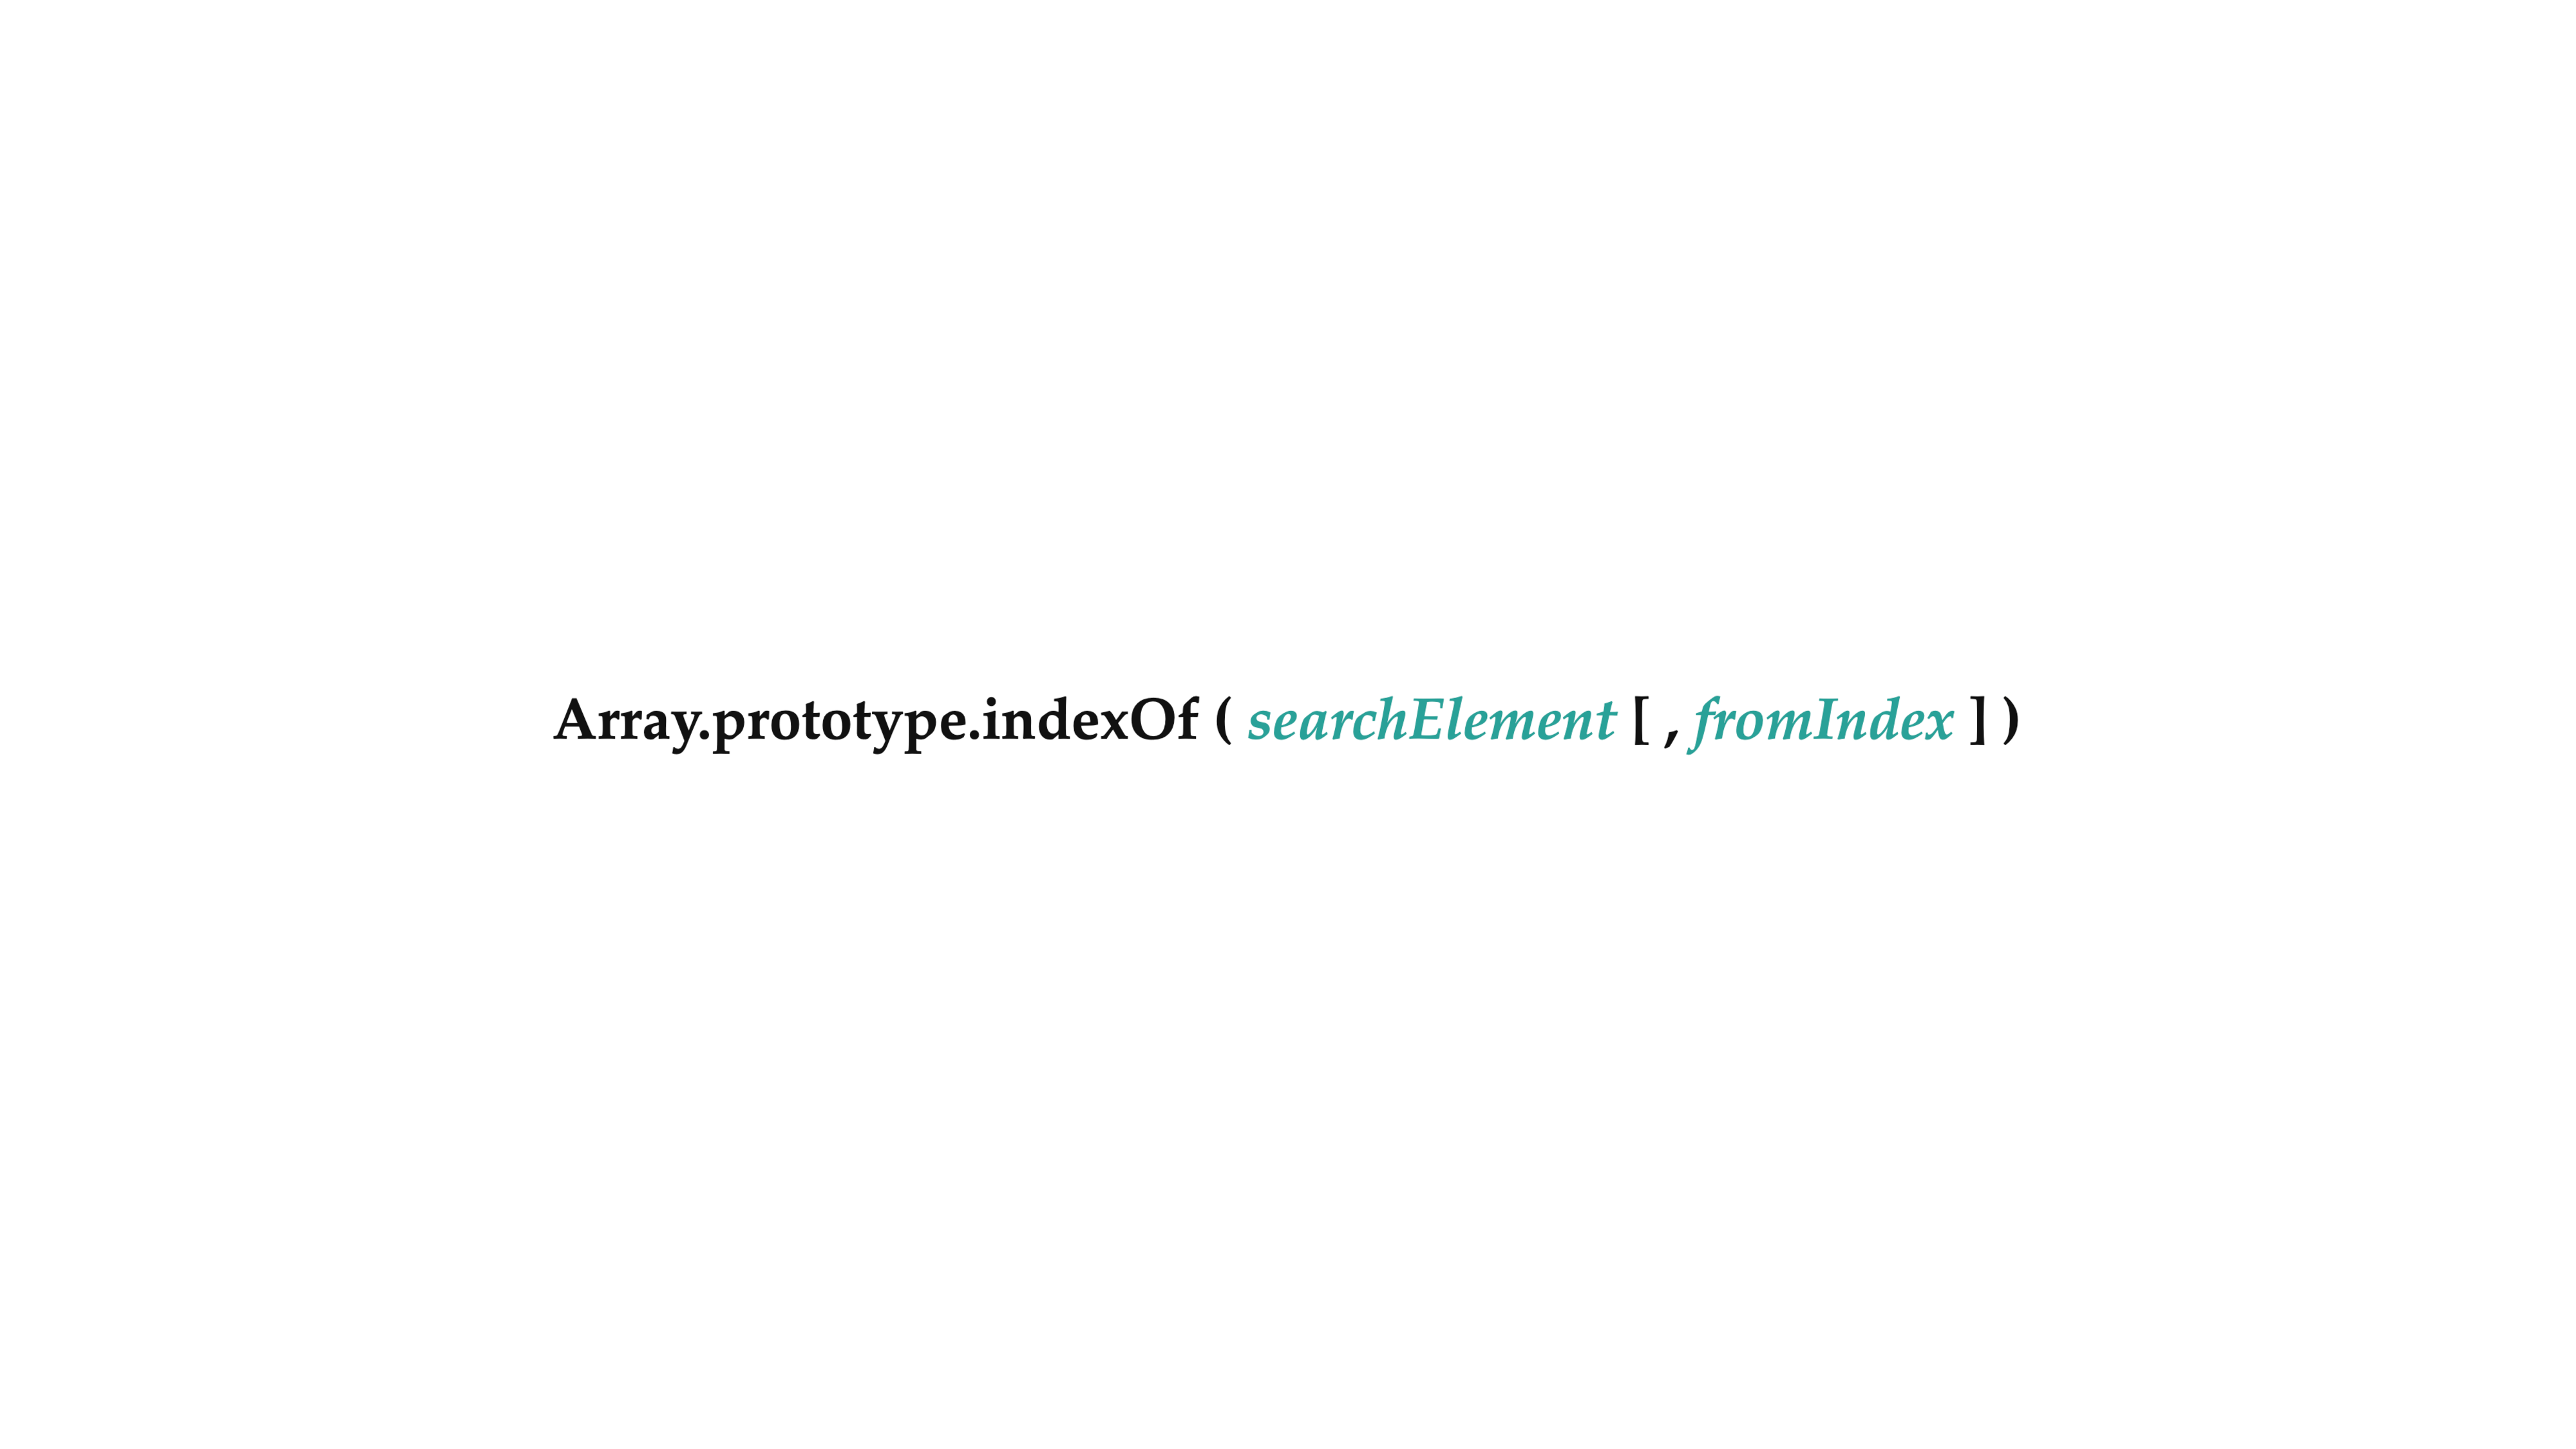
\includegraphics[width=0.4\textwidth]{img/array-indexof.pdf}
\end{figure}

For example, consider the above \code{Array.prototype.indexOf} function for
JavaScript array objects.  It takes one parameter \textit{searchElement} that
denotes the element we want to search and one more optional parameter
\textit{fromIndex} to change the searching scope.  Thus, the synthesizer passes
one or two arguments with an array object or \code{null} as the \code{this}
object as follows:
\begin{lstlisting}[style=myJSstyle]
Array.prototype.indexOf.call(new Array(), 0);
Array.prototype.indexOf.call(new Array(), 0, 0);
Array.prototype.indexOf.call(null, 0);
Array.prototype.indexOf.call(null, 0, 0);
\end{lstlisting}
Moreover, \code{Array} itself is also not only a built-in function but also
a built-in constructor with an optional single argument or variable arguments.
Thus, we synthesize the following six programs for \code{Array}:
\begin{lstlisting}[style=myJSstyle]
Array();      Array(0);      Array(0, 0);
new Array();  new Array(0);  new Array(0, 0);
\end{lstlisting}

\subsection{Target Selector}

At the first step, \textsf{Target Selector} initializes the program pool with
the seed programs synthesized by \textsf{Seed Synthesizer}.  Then, it repeatedly
picks a target program that will be mutated in \textsf{Program Mutator}.  To
focus on increasing the semantics coverage, we use the branch coverage
of the current program pool when selecting the target program.

For example, Figure~\ref{fig:example-algo} is an excerpt of the \textbf{Abstract
Equality Comparison} algorithm that describes the semantics of non-strict
equality comparison operators (\code{==} or \code{\!=}).  Assume that the
following programs are the current program pool:
\begin{lstlisting}[style=myJSstyle]
1 + 2;  true == false;  0 == 1;
\end{lstlisting}
In this case, all pairs of left- and right-hand sides of the equality operator
in the current program pool have the same typed values.  Thus, in the first step
in the algorithm, the condition ``Type($x$) is the same as Type($y$)'' is always
true and the false branch is not covered.  To cover this false branch, the
\textsf{Target Selector} selects a program that passes the true branch such as
\code{true == false;} or \code{0 == 1;}.  If the program \code{true == false;} is
selected and mutated to \code{42 == false;} by \textsf{Program Mutator}, the
new program covers more semantics thus the program pool is extended as follows:
\begin{lstlisting}[style=myJSstyle]
1 + 2;  true == false;  0 == 1;  42 == false;
\end{lstlisting}
Then, \textsf{Target Selector} has more choices of branches in steps 2, 3, 10,
and 11 to select next target program.  When it targets the branch in the step
10, it selects the code \code{42 == false;} as the target program.  In the same
way, \textsf{Target Selector} iterates this process until the semantics coverage
is converged.

\subsection{Program Mutator}

Given a target program, \textsf{Program Mutator} repeatedly tries to mutate the
target program to another program to increase semantics coverage.  One trial
consists of the following steps.  First, it randomly selects one of five
mutation methods and produces a mutated program.  If it is a new program, the
mutator checks whether it increases the semantics coverage of the program pool.
If it succeeds, the mutated program is added to the program pool.  This process
is repeated at most pre-defined maximum trial number.  Now, we explain five
mutation methods used in \textsf{Program Mutator}.


\subsubsection{Random Mutation}
The first approach is a na\"ive method that randomly selects a statement, a
declaration, or an expression in a given program and mutates the selected the
syntax tree.  We utilize the non-recursive synthesizer to extract set of syntax
trees and randomly selects and inserts one of them in the target position.
For example, assume that the expression \code{1} is selected in the program
\code{var x = 1 + 2;}.  Then, the left-hand side of the addition operator
(\code{+}) will be mutated by a random expression such as \code{var x = true +
2;}.


\subsubsection{Nearest Syntax Tree Mutation}
This approach focuses on a branch whose true(false) branch is covered by the
given target program but the other false(true) branch is not covered by any
programs in the current program pool.  To increase the semantics coverage by
targeting the uncovered part, it finds the nearest syntax tree that reaches the
target branch in the given program.  Then, the nearest syntax tree is mutated by
a random syntax tree derivable from the same syntax production.  For example,
consider the following JavaScript program:
\begin{lstlisting}[style=myJSstyle]
var x = '' + (1 == 2);
x *= 3 / true;
\end{lstlisting}
Assume that any programs in the current program pool cannot cover the true
branch in the first step of the \textbf{Abstract Equality Comparison} algorithm
in Figure~\ref{fig:example-algo}.  The above program covers only the false
branch in the first step thus the mutator targets this branch and finds the
nearest syntax tree.  Because the nearest part is \code{1 == 2} in the program,
this approach tries to mutate only \code{1 == 2} not other syntax trees.


\subsubsection{String Substitutions}
We utilize the literals as values in ECMAScript for diversity of JavaScript
values in generated tests.  Most of literals existed in the specification
represent the corner case values such as \code{-0}, \code{Infinity}, or
\code{NaN}.  However, in some cases, specific strings are necessary to cover
some semantics.  For example, the algorithm of [[DefineOwnProperty]] internal
method of array exotic objects has different semantics depending on whether its
parameter \code{P} is a string \code{"length"} or not.  Thus, we collects all
string literals used in the conditions in any algorithms in ES11 and randomly
substitutes with an expression with one of them.


\subsubsection{Object Substitutions}
Some abstract algorithms in ECMAScript try to access some properties of an
object using \textbf{HasProperty}, \textbf{GetMethod}, \textbf{Get}, and
\textbf{OrdinaryGetOwnProperty} algorithms.  In this case, objects having such
properties are necessary to handle such algorithms.  Thus, we collects all
touched algorithms including any invocations of such property access algorithms
similar with string substitutions.  For each invocation, we collects string
literals and symbols used as its arguments.  Based on collected string values
and symbols, we randomly generate object literals and replace a randomly
selected expression with the generated object.  For example, the following
program touches two algorithms \textbf{ToPrimitive} that has the invocation of
\textbf{GetMethod} with the symbol \code{Symbol.toPrimitive} and
\textbf{ToPropertyDescriptor} that has the invocation of \textbf{Get} with
string literals \code{"get"}, \code{"set"}, \code{"value"}, \code{"writable"},
\code{"enumerable"}, and \code{"configurable"}.
\begin{lstlisting}[style=myJSstyle]
Object.defineProperty({}, 'p', 42);
\end{lstlisting}
Thus, the mutator mutates a randomly selected expression in the program with a
randomly generated object having properties whose keys are extracted symbols and
string values.  If the expression \code{42} is selected, it might increase the
semantics coverage with a high probability because the generated object could be
a specific property descriptor.


\subsubsection{Statement Insertion}
To synthesize more complex programs, the mutator supports to insert a random
statement into the end of a randomly selected statement list such as in
the top-level code, block statements, or function bodies.  We also utilize the
non-recursive synthesizer to synthesize a random statement with a pre-defined
special statements.  The special statements have better potential to change the
execution path, such as function calls, \code{return}, \code{break}, and
\code{throw}, and they are selected with a higher probability than fully random
statements synthesized by non-recursive synthesizer.  For example, assume the
the function body in the following program is selected and the \code{throw 42;}
is the new statement.
\begin{lstlisting}[style=myJSstyle]
function f() {} f();            // original
function f() { throw 42; } f(); // mutated
\end{lstlisting}
Then, the mutated program throws an exception during a function call and it is
helpful to cover different semantics related to control statements.

\subsection{Assertion Injector}

After generating JavaScript programs, \textsf{Assertion Injector} injects
assertions to them based on the final state of the program according to
ECMAScript.  It first obtains the final state of a given program from the
mechanized specification and injects six different kinds of assertions to the
program.  We carefully implement helper functions for assertions in JavaScript
not to affect the semantics of the original program and inject them in the front
of the given program.  Moreover, in order to check the final state after
executing all asynchronous jobs assigned in the job queue, we enclose assertions
with \code{setTimeout} to wait 100ms when the program uses asynchronous features
such as \code{Promise} or \code{async}:
\begin{lstlisting}[style=myJSstyle]
// a given program
setTimeout(() => {
  // injected assertions
}, 100)
\end{lstlisting}


\subsubsection{Exceptions}

JavaScript supports both internal exceptions, such as \code{SyntaxError} and
\code{TypeError}, and custom exceptions with the keyword \code{throw}.  We could
catch such exceptions using \code{try-catch} statements.  However, it might
change the semantics of a given program.  For example,
\begin{lstlisting}[style=myJSstyle]
var x; function x() {}
\end{lstlisting}
does not throw any exception but
\begin{lstlisting}[style=myJSstyle]
try { var x; function x() {} } catch (e) {}
\end{lstlisting}
throws a \code{SyntaxError} because the same name of a variable and a function
declaration is not allowed in \code{try-catch} blocks.

To resolve this problem, we utilize the comment in the first line.  If the
program throws an internal exception, we tag its name in the comment.
Otherwise, we tag \code{Throw} for a custom exception and \code{Normal} for
the normal termination.  Using the tag in the comment, we checked the execution
result of the program in each engine.  For example, ES11 says that the example
JavaScript program in Figure~\ref{fig:example-algo} normally terminates thus the
program is modified as follows:
\begin{lstlisting}[style=myJSstyle]
// Normal
var obj = { valueOf: () => { throw 'err'; } };
var result = 42 == obj;
\end{lstlisting}


\subsubsection{Variable Values}

We injected assertions that compare values stored in variables with expected
values.  To focus on newly introduced variables during the execution, we do not
compare pre-defined variables such as built-in objects.  It detects variables
introduced by not only variable declarations (\code{var}) but also lexcial
(\code{let} or \code{const}) and function declarations.  We discriminate
\code{-0} and \code{+0} using division by zero because \code{-0/0} and
\code{+0/0} produce positive and negative infinity values, respectively.  For
object values, we use other assertions to deeply check them.  For example, the
following code is an example that checks whether the value of the variable
\code{x} is \code{3}.
\begin{lstlisting}[style=myJSstyle]
var x = 1 + 2;
$assert.sameValue(x, 3);
\end{lstlisting}


\subsubsection{Object Values}

To check the equality between two object values, we keep the representative path
for each object.  If the injector meets an object in the first time, it injects
assertions for its properties will be explained in the remaining the section and
stores the current path.  Otherwise, the injector adds assertions to compare the
current path and the representative path.
\begin{lstlisting}[style=myJSstyle]
var x = {}, y = {}, z = { p: x, q: y };
$assert.sameValue(z.p, x);
$assert.sameValue(z.q, y);
\end{lstlisting}
For example, in the above code, the injector meets two different new objects
stored in the variables \code{x} and \code{y} thus it stores the paths \code{x}
and \code{y}.  Then, the object in \code{z} is also a new object but its
properties \code{z.p} and \code{z.q} stores already visited objects.  Thus, the
injector inserts two assertions that check whether \code{z.p} and \code{x} have
a same object and \code{z.q} and \code{y} have a same object.  To handle
built-in objects, we store all paths of built-in objects before traversing the
state.


\subsubsection{Property Descriptors}

JavaScript supports two different kinds of object properties: \textit{data
property} and \textit{accessor property}.  Each property consists of four
different attributes [[Value]], [[Writable]], [[Enumerable]], and
[[Configurable]] for data properties and [[Get]], [[Set]], [[Enumerable]], and
[[Configurable]] for accessor properties.  We could access them using the
\code{Object.getOwnPropertyDescriptor} built-in function.  It takes an object
and a value that represents a property key, and returns an object that
represents the property descriptor.  We implement a helper
\code{\$verifyProperty} to check attributes of each property for each object.
For example, the following code checks attributes of the data property
\code{x.p}.
\begin{lstlisting}[style=myJSstyle]
var x = { p: 42 };
$verifyProperty(x, "p", {
  value: 42.0,
  writable: true,
  enumerable: true,
  configurable: true
});
\end{lstlisting}


\subsubsection{Property Keys}

Since ECMAScript 2015 (ES6), the order between property keys in objects is
defined in the specification.  Thus, we check the order by using the
\code{Reflect.ownKeys} built-in function that returns an array that consists of
own property keys for a given object.  We implement a helper
\code{\$assert.compareArray} that takes two different arrays and compare their
length and contents.  For example, the following program is an example that
checks the property keys and their order of the object in \code{x}.
\begin{lstlisting}[style=myJSstyle]
var x = {
  [Symbol.match]: 0,
  p: 0, 3: 0, q: 0
}
$assert.compareArray(
  Reflect.ownKeys(x),
  ['3', 'p', 'q', Symbol.match]
);
\end{lstlisting}


\subsubsection{Internal Methods and Slots}

JavaScript objects have internal methods and slots that we cannot direcly
access.  However, several internal methods and slots are accessible using
indirect ways.  We target four internal slots with their appropriate indirect
getters as follows:
\[
  \begin{array}{|l|l|}\hline
    \telembf{|c|}{Name}   & \telembf{c|}{Indirect Getter}\\\hline
    \text{[[Prototype]]}  & \code{Object.getPrototypeOf(x)}\\\hline
    \text{[[Extensible]]} & \code{Object.isExtensible(x)}\\\hline
    \text{[[Call]]}       & \code{typeof f === 'function'}\\\hline
    \text{[[Construct]]}  & \code{Reflect.construct(function()\{\},[],x)}\\\hline
  \end{array}
\]

The internal slot [[Prototype]] represents the prototype object of an object.
We extracts it using a built-in function \code{Object.getPrototypeOf}.  In the
similar way, we use \code{Object.isExtensible(x)} for [[Extensible]] slot.  The
internal methods [[Call]] and [[Construct]] represents whether a given object is
a function or a constructor.  However, methods stored in [[Call]] and
[[Construct]] are not JavaScript values thus we only check the their existence
using two helpers \code{\$assert.callable} and \code{\$assert.constructable}.  For
[[Call]] method, we use the \code{typeof} operator because it returns the string
\code{"function"} if and only if the given value is an object has the [[Call]]
internal method.  For [[Construct]] method, we use the \code{Reflect.construct}
built-in function that checks the existence of [[Construct]] methods and invokes
it.  To preserve the current state, we pass a given object as the third argument
to only check the existence of [[Construct]] and pass another dummy function
\code{funcion(){}} as the first argument whose [[Construct]]
invoked by \code{Reflect.construct}.  For example, the following code describes
how the injector injects assertions related to internal methods and slots:
\begin{lstlisting}[style=myJSstyle]
function f() {}
$assert.sameValue(Object.getPrototypeOf(f),
                  Function.prototype);
$assert.sameValue(Object.isExtensible(x), true);
$assert.callable(f);
$assert.constructable(f);
\end{lstlisting}

\subsection{Bug Localizer}

The bug detection and localization phase uses the execution results of
given conformance tests on multiple JavaScript engines.
If a small number of engines fail in running a specific conformance test,
the engines may have bugs causing the test failure.
If most engines fail for a test, the test may be incorrect,
which implies a bug in the specification.

When we have a set of failed test cases that may contain bugs of an engine or a
specification, we classify the test cases using their failure
messages and give ranks between possible buggy program elements to localize the bug.
We use Spectrum Based Fault Localization (SBFL)~\cite{sbfl-survey},
which is a ranking technique based on likelihood of being faulty for each
program element.  We use the following formula called $ER1_b$,
which is one of the best SBFL formulae theoretically analyzed by Xie et al.~\cite{er1b}:
\[
  {n_{\mbox{\emph{\scriptsize ef}}}} -
  {
    {n_{\mbox{\emph{\scriptsize ep}}}}
    \over
    {n_{\mbox{\emph{\scriptsize ep}}} + n_{\mbox{\emph{\scriptsize np}}} + 1}
  }
\]
where $n_{ef}$, $n_{ep}$ , $n_{nf}$, and $n_{np}$ represent the number of test
cases; subscripts ${}_e$ and ${}_n$ respectively denote whether a test case touches a
relevant program element or not, and subscripts ${}_f$ and ${}_p$
respectively denote whether the test case is failed or passed.

We use abstract algorithms of ECMAScript as program elements used for SBFL.
To improve the localization accuracy, we use method-level aggregation~\cite{fluccs}.
It first calculates SBFL scores for algorithm steps and aggregates
them up to algorithm-level using the highest score among those from steps of each algorithm.


\section{Evaluation}\label{sec:eval}

\begin{figure*}[t]
  \centering
  \begin{subfigure}[t]{0.48\textwidth}
    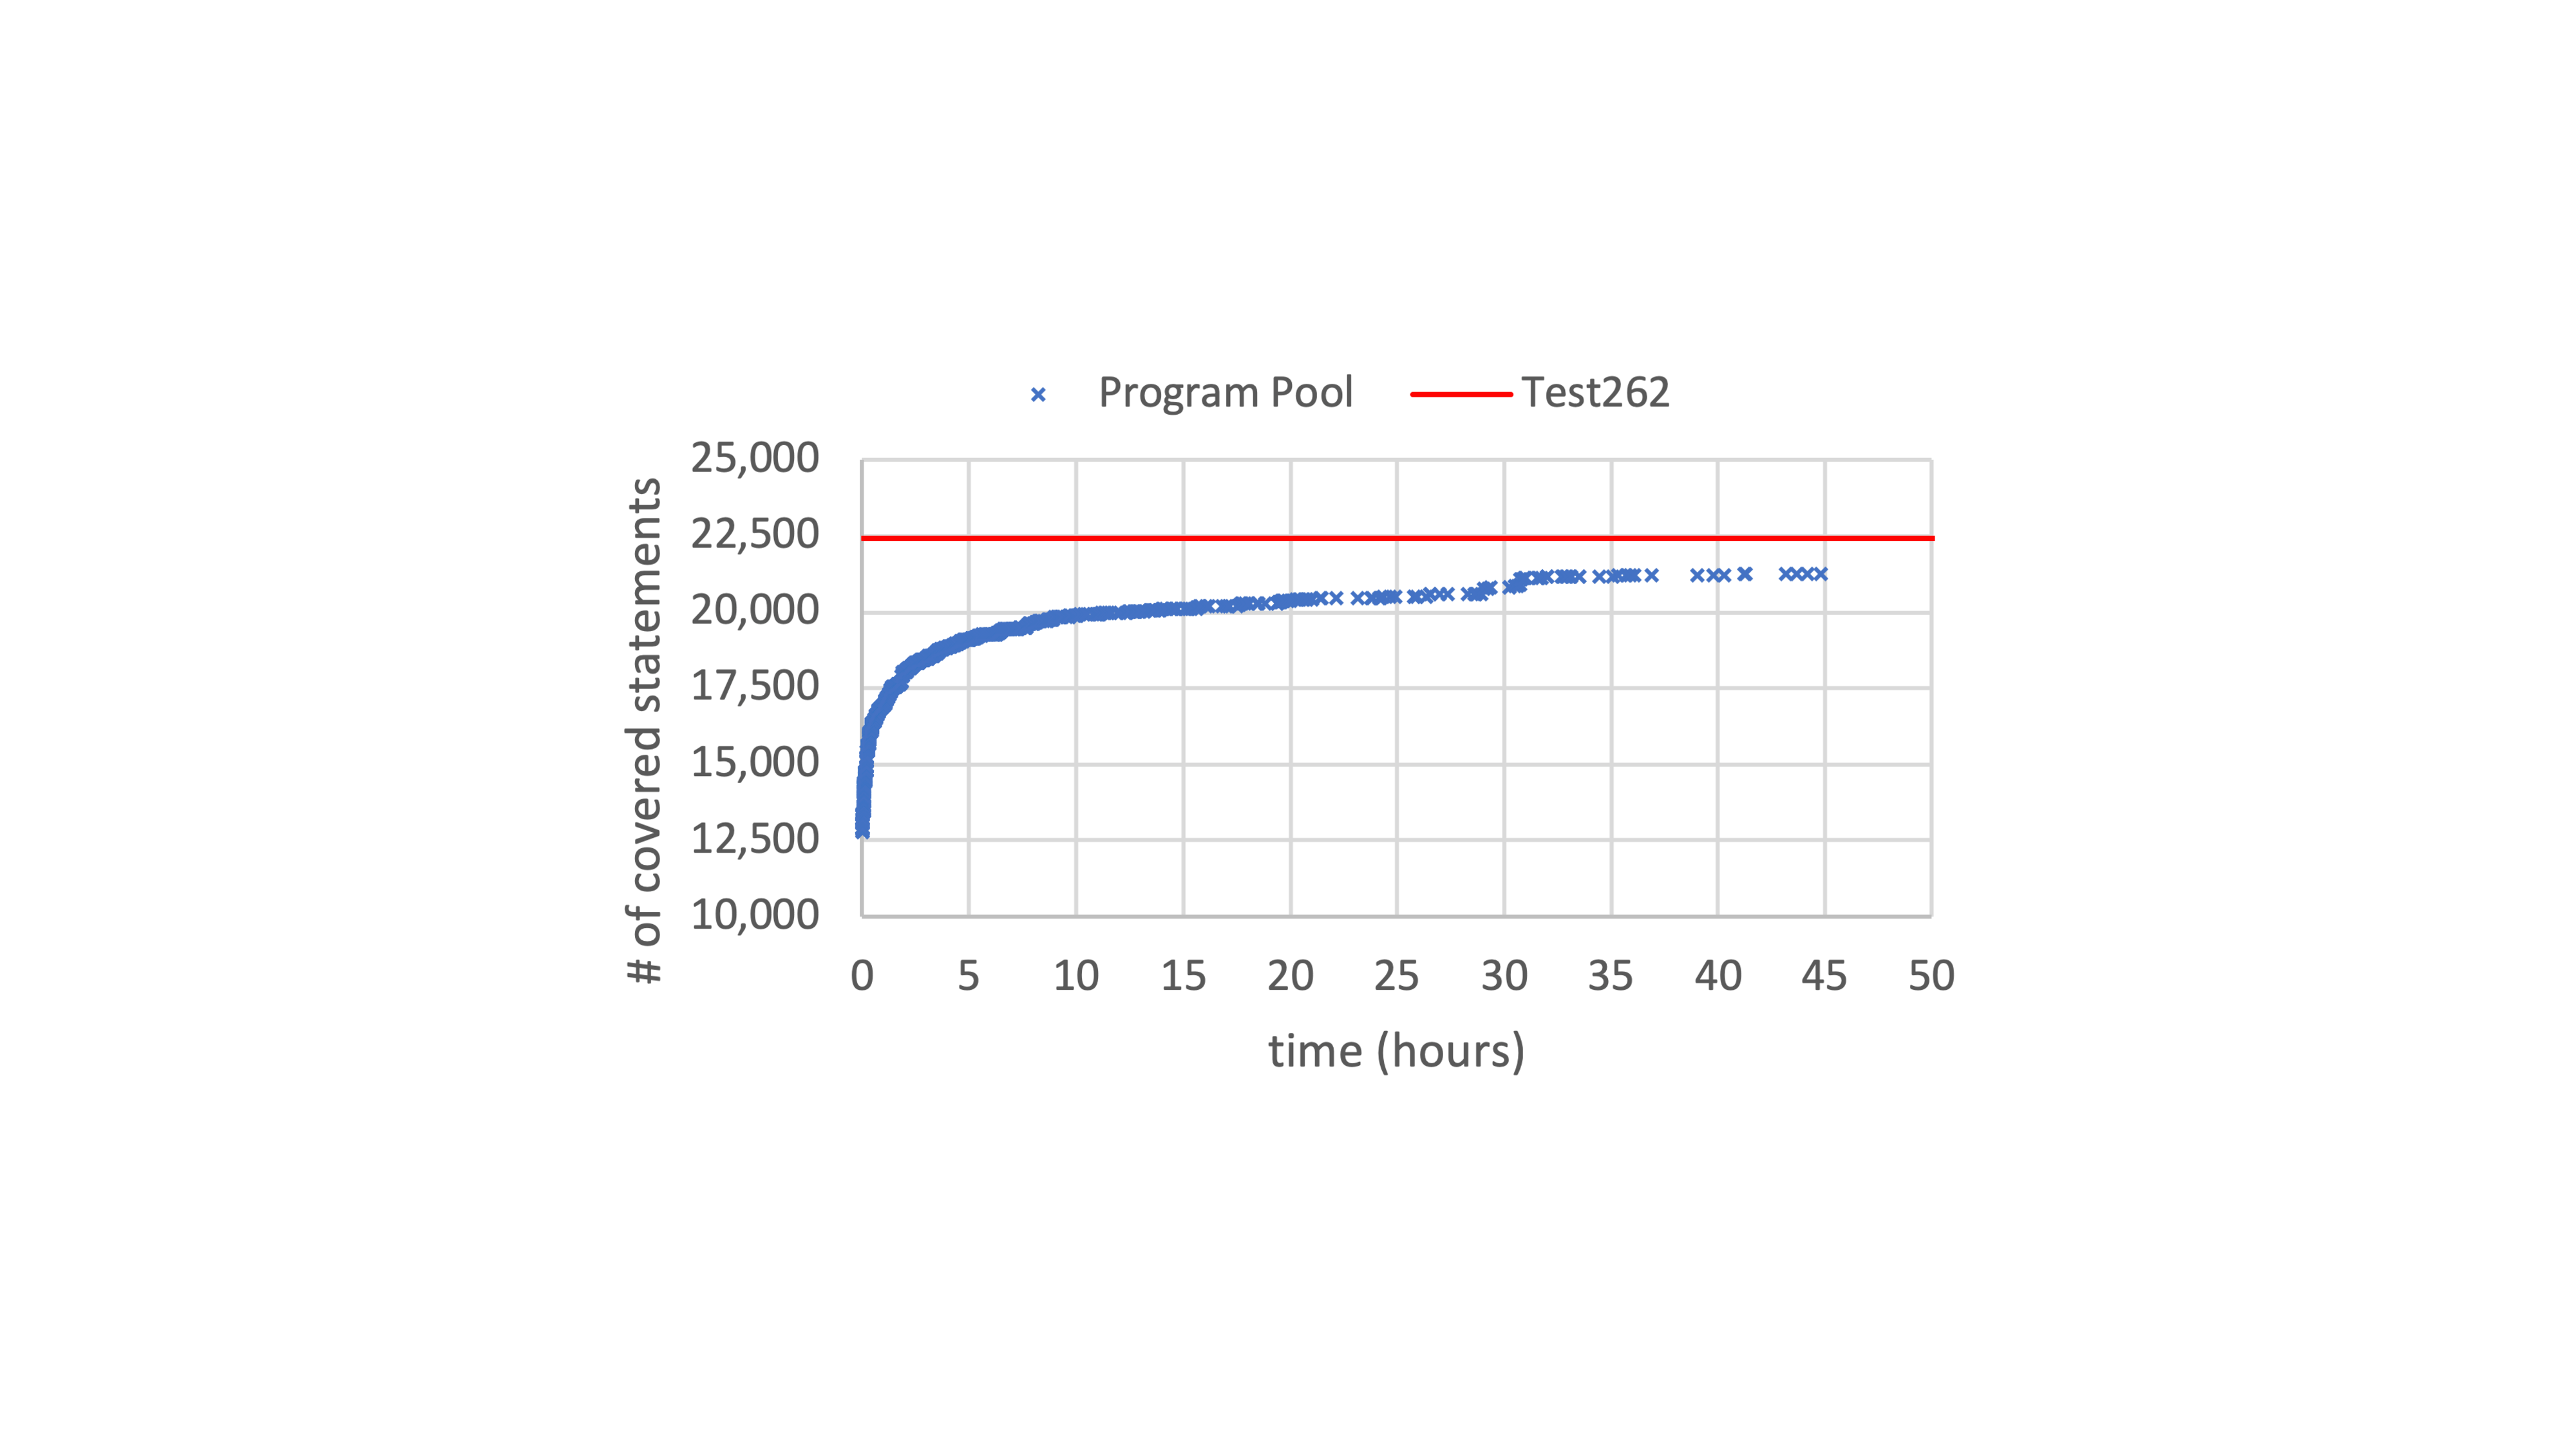
\includegraphics[width=\textwidth]{img/stmt-coverage.pdf}
    \caption{The statement coverage}
    \label{fig:stmt-coverage}
  \end{subfigure}
  \quad
  \begin{subfigure}[t]{0.48\textwidth}
    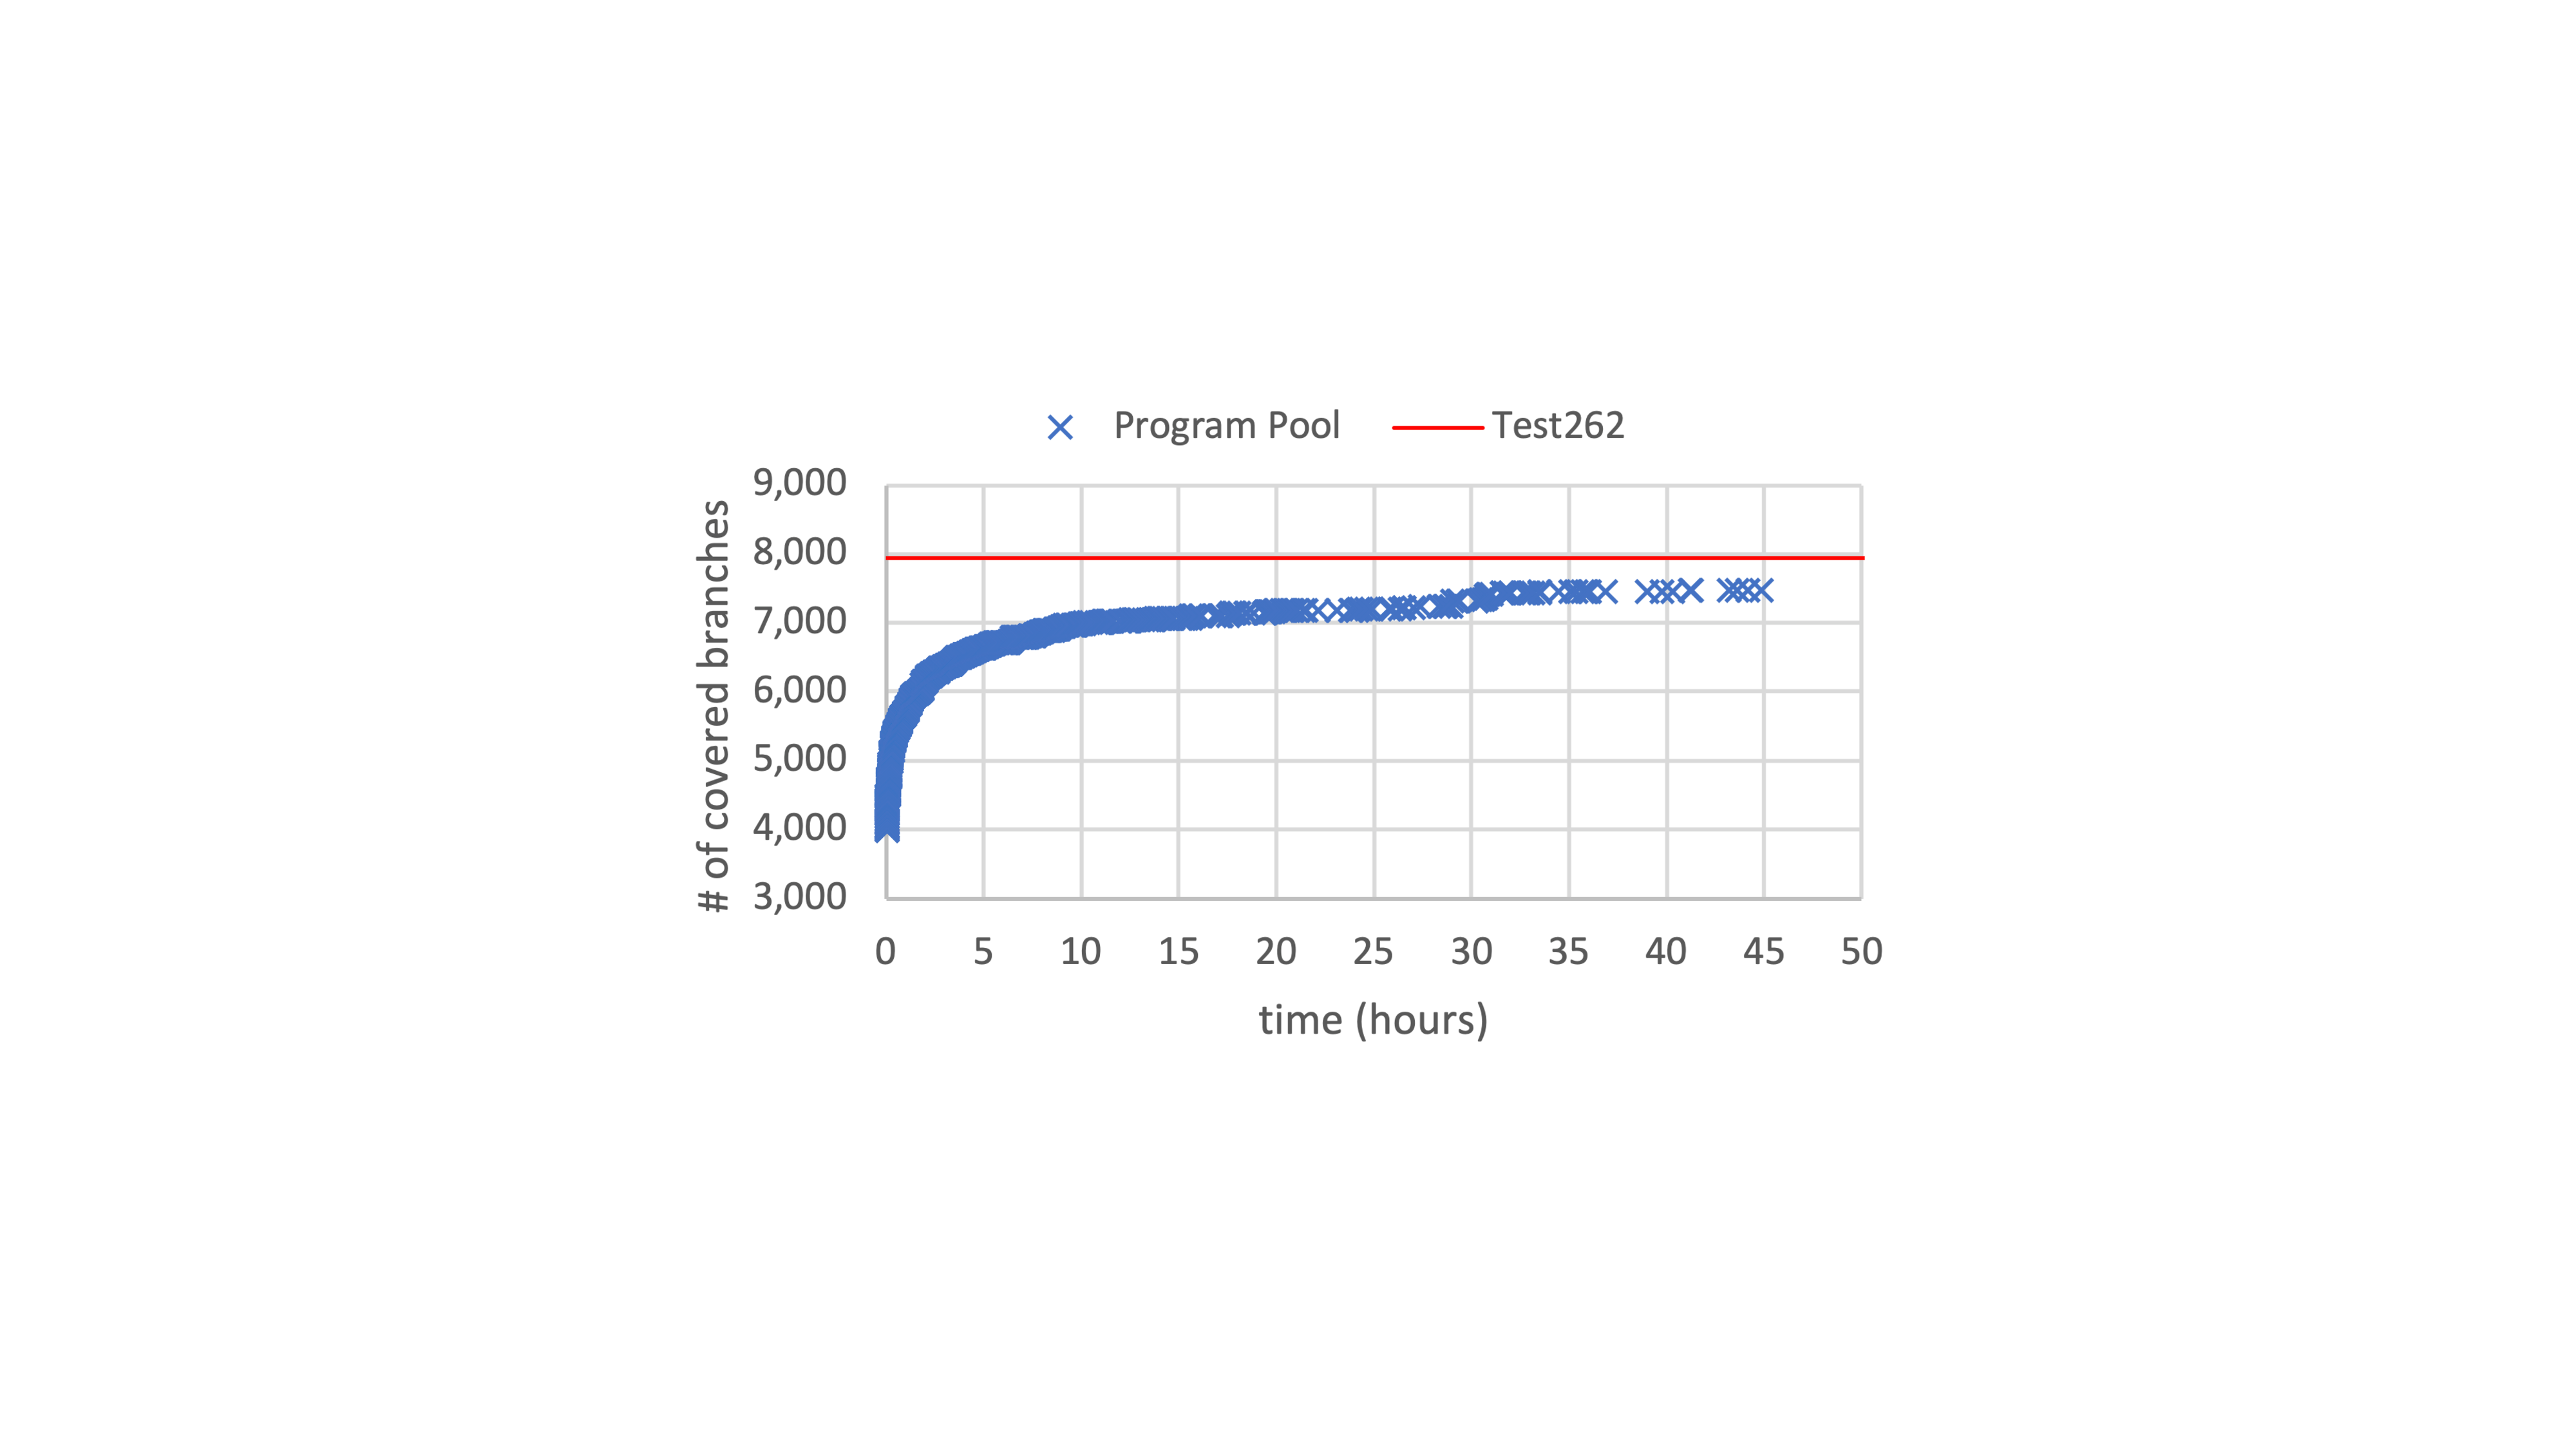
\includegraphics[width=\textwidth]{img/branch-coverage.pdf}
    \caption{The branch coverage}
    \label{fig:branch-coverage}
  \end{subfigure}
  \caption{The semantics coverage changes during the test generation phase}
  \label{fig:sem-coverage}
  \vspace*{-1em}
\end{figure*}

To evaluate $\tool$ that performs the $N$+1-version differential testing of JavaScript
engines and specification, we applied our tool to four JavaScript engines that
fully support modern JavaScript features and the most recent specification,
ECMAScript 2020 (ES11, 2020).  We targeted the following four JavaScript
engines and all of them supports
ES11\footnote{https://github.com/graalvm/graaljs\#current-status}\footnote{https://bellard.org/quickjs/}\footnote{https://blog.moddable.com/blog/xs10/}\footnote{https://v8.dev/}:
\begin{itemize}
  \item \textbf{GraalJS(v20.1.0):} A JavaScript implementation built on
    GraalVM\cite{graaljs}, which is a Java Virtual Machine (JVM) based on
    HotSpot/OpenJDK developed by Oracle.
  \item \textbf{QuickJS(2020-04-12):} A small and embedded JavaScript engine developed by
    Fabrice Bellard and Charlie Gordon\cite{qjs}.
  \item \textbf{Moddable XS(v10.2.1):} A JavaScript engine at the center of the Moddable
    SDK\cite{xs}, which is a combination of development tools and runtime
    software to create applications for micro-controllers.
  \item \textbf{V8(v8.5):} The Google's open source high-performance JavaScript and
    WebAssembly engine\cite{v8}, written in C++.
\end{itemize}
To extract mechanized specification from ECMAScript, we utilize the tool
$\jiset$, which is a JavaScript IR-based semantics extraction toolchain.
automatically extracted from a given ECMAScript.  To focus on the semantics of
core JavaScript semantics, we only consider the semantics of strict mode
JavaScript codes that pass syntax checking including the EarlyError rules.  To
filter out the JavaScript codes that are not strict or fail the syntax checking,
we utilize the syntax checker of the most reliable JavaScript engine, V8.
We performed our experiments on a machine equipped with 4.0GHz Intel(R) Core(TM)
i7-6700k and 32GB of RAM (Samsung DDR4 2133MHz 8GB*4).  We evaluated our tool
based on the following four research questions:
\begin{itemize}
  \item {\bf RQ1 (Coverage of Generated Tests)} The semantics coverage compared
    to Test262, the manually written official conformance test suite for
    ECMAScript.
  \item {\bf RQ2 (Accuracy of Bug Localization)} The accuracy of bug locations
    pointed by \mytextsf{Bug Localizer} compared to the actual bug locations.
  \item {\bf RQ3 (Bug Detection in JavaScript Engines)} The number of bugs in
    four JavaScript engines detected by $\tool$.
  \item {\bf RQ4 (Bug Detection in ECMAScript)} The number of specification bugs
    in ES11 detected by $\tool$.
\end{itemize}


\subsection{Coverage of Generated Tests}

For the first step, we synthesize seed programs via \mytextsf{Seed Synthesizer}
based on the syntax of ES11.  It synthesizes \inred{1,112} JavaScript programs
in about \inred{10} seconds and covers \inred{97.25\% (395/406)} of reachable
alternatives in syntax productions.  The seed programs becomes the initial
program pool and it gradually grows via \mytextsf{Target Selector} and
\mytextsf{Program Mutator}.  Figure~\ref{fig:sem-coverage} shows the change of
semantics coverage of the program pool during the iterative process in
\inred{50} hours.  The left and right graphs show the statement and branch
coverage, respectively.  The red line denotes the coverage of tests of Test262,
dark gray X marks denote tests generated from ES11, and blue O marks denote
tests generated from ES11 after fixing bugs detected by our tool.  For the
statement coverage, \inred{29,728} statements exist in ES11 and tests in Test262
covers \inred{22,425 (75.43\%)} statements.  The initial program pool covers
\inred{12,766 (42.94\%)} statements and the final program pool covers
\inred{21,249 (71.48\%)} and \inred{21,249 (71.48\%)} statements before and
after fixing bugs, respectively.  For branch coverage, \inred{11,448} branches
exist in ES11 and tests in Test262 covers \inred{7,944 (69.39\%)} branches.  The
initial program pool covers \inred{3,986 (34.82\%)} branches and the final
program pool covers \inred{7,476 (65.30\%)} and \inred{7,476 (65.30\%)} branches
before and after fixing bugs.

\begin{table}
  \caption{The number of successes and covered branches for mutation methods}
  \label{table:mutation-method}
  \vspace*{-1em}
  \small
  \[
    \begin{array}{l?r|r}
      \telembf{c?}{Mutation Methods}      & \telembf{c}{Success}  & \telembf{c}{Branch (Avg.)}\\\toprule\\[-1.4em]
      \text{Nearest Syntax Tree Mutation} & \rtext{436}           & \rtext{1,450 (3.33)}\\\hline
      \text{Random Mutation}              & \rtext{320}           & \rtext{910   (2.84)}\\\hline
      \text{Statement Insertion}          & \rtext{201}           & \rtext{672   (3.34)}\\\hline
      \text{Object Substitution}          & \rtext{162}           & \rtext{453   (2.80)}\\\hline
      \text{String Substitution}          & \rtext{4}             & \rtext{5     (1.25)}\\\hline
      \hline
      \telembf{c?}{Total}                 & \rtext{1,123}         & \rtext{3,490 (3.11)}\\
    \end{array}
  \]
  \vspace*{-1.5em}
\end{table}

Table~\ref{table:mutation-method} shows the number of successes and covered
branches for each mutation method during the test generation phase.  In total,
$\tool$ succeeds to synthesize \inred{1,123} programs that covers \inred{3,490}
more branches than the initial program pool.  Among five mutation methods, the
nearest syntax tree mutation is the most contributed method (\inred{436}
successes and \inred{1,450} covered branches) and the least one is the string
substitution (\inred{4} successes and \inred{5} covered branches).  On average,
\inred{3.11} branches are covered by one successful mutation.

Finally, $\tool$ generates \inred{X,XXX} JavaScript programs and the average
length of generated programs is \inred{XX.XX}.  After injecting assertions by
\mytextsf{Assertion Injector}, generated programs become conformance tests and
their average length is \inred{XXX.XX}.  Compared to Test262, the number of
generated tests are much smaller and their sizes also shorter than that of tests
in Test262.  Test262 provides \inred{XX,XXX} tests for the same range of
semantics and their average size is \inred{XXX.XX}.


\subsection{Accuracy of Bug Localization}

\begin{figure}[t]
  \centering
  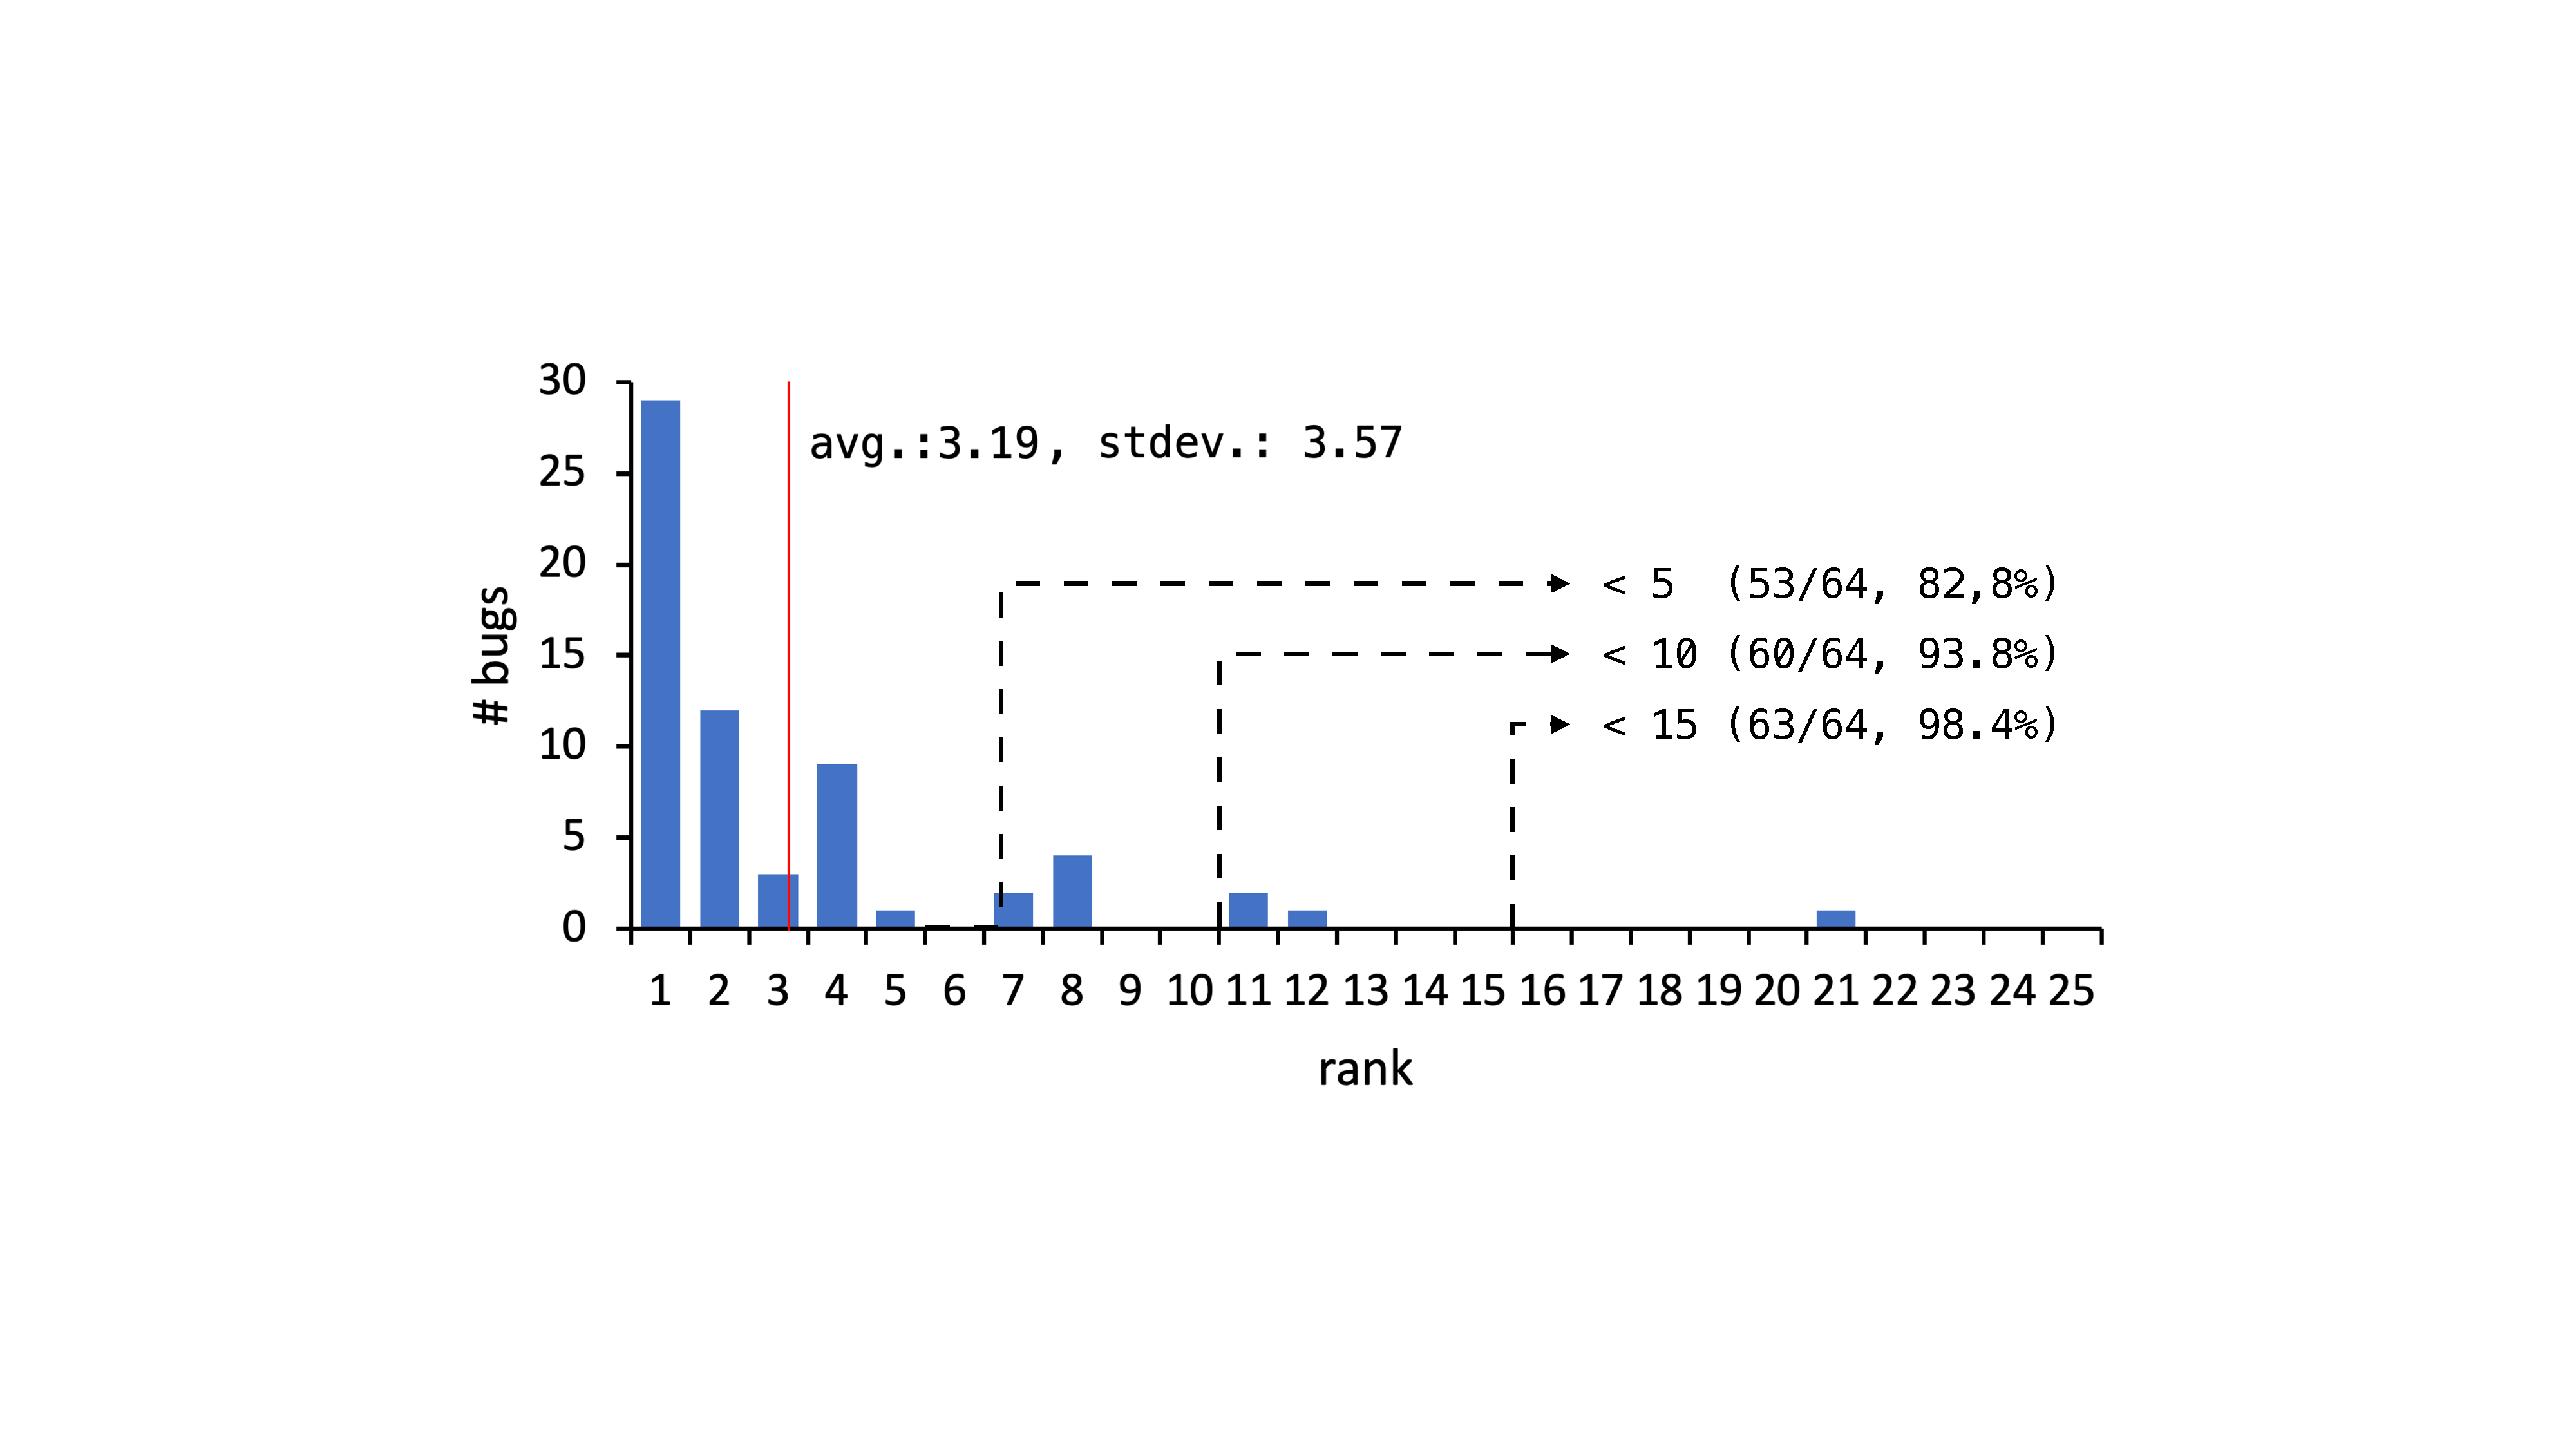
\includegraphics[width=0.48\textwidth]{img/localize.pdf}
  \caption{Ranks of actual buggy alogrithms in results of \mytextsf{Bug Localizer}
    for bugs detected by $\tool$}
  \label{fig:localize}
  \vspace*{-1em}
\end{figure}

We executed the generated conformance tests on four different JavaScript engines
to find engine or specification bugs.  We utilize the majority of execution
results to assort bugs as engine or specification bugs.  If most of engines
fails to a specific conformance test, we believe that the failure of the test
represents the correct semantics.  Thus, we suspect engines passing the test and
the specification of containing bugs related to the test.  Otherwise, we assume
that bugs exist in engines failing the test.  We manually checked the detected
bugs whether they are actually engine bugs or specification bugs.  The following
table shows the number of engines failing tests related to each bug.

\begin{table}[H]
  \centering
  \vspace*{-1em}
  \small
  \[
    \begin{array}{l?r|r|r|r?r?r}
      \telembf{c?}{\# Fails} &
      \telembf{c}{1} &
      \telembf{c}{2} &
      \telembf{c}{3} &
      \telembf{c?}{4} &
      \telembf{c?}{Total} &
      \telembf{c}{Avg.} \\\toprule\\[-1.4em]

      \text{Engine Bugs}  & \inred{-} & \inred{-} & \inred{-} & \inred{-} & \inred{39} & \inred{1.3}\\\hline
      \text{Spec. Bugs}   & \inred{-} & \inred{-} & \inred{-} & \inred{-} & \inred{7} & \inred{3.8}
    \end{array}
  \]
  \vspace*{-1em}
\end{table}

According to the table, our assumption seems to be reliable because tests
related to engine bugs failed in \inred{1.3} engines on average.  For
specification bugs, the related tests failed in \inred{3.8} engines on average.

Based on results of conformance tests on four JavaScript engines, we localize
the specification or engine bugs on the semantics of ES11.  We detected
\inred{-} bugs and Figure~\ref{fig:localize} shows the ranks of their actual
buggy algorithms in results of \mytextsf{Bug Localizer}.  The average rank is
\inred{-}, and \inred{-}\% of buggy algorithms are ranked in less than 5,
\inred{-}\% in less than 10, and \inred{-}\% in less than 15.  Among \inred{-}
bugs, locations of \inred{-} bugs are ranked in more than \inred{-}.  It shows
the limitation of the statistical fault localization that have low accuracy of
localization for bugs caused by missing statements.  For example, \inred{TODO:
example}.



\subsection{Bug Detection in JavaScript Engines}

\begin{table}
  \caption{The number of engine bugs detected by $\tool$}
  \label{table:engine-bug}
  \vspace*{-1em}
  \small
  \[
    \begin{array}{l?r|r|r|r|r|r|r?r}
      \telembf{@{}c@{~}?}{Engines} &
      \telemsf{@{~}c@{~}|}{Exc} &
      \telemsf{@{~}c@{~}|}{Crash} &
      \telemsf{@{~}c@{~}|}{Var} &
      \telemsf{@{~}c@{~}|}{Obj} &
      \telemsf{@{~}c@{~}|}{Desc} &
      \telemsf{@{~}c@{~}|}{Key} &
      \telemsf{@{~}c@{~}?}{In} &
      \telembf{@{~}c@{}}{Total}\\\toprule\\[-1.4em]

      \text{GraalJS}      & \inred{-} & \inred{-} & \inred{-} & \inred{-} & \inred{-} & \inred{-} & \inred{-} & \inred{10}\\\hline
      \text{QuickJS}      & \inred{-} & \inred{-} & \inred{-} & \inred{-} & \inred{-} & \inred{-} & \inred{-} & \inred{6}\\\hline
      \text{Moddable XS}  & \inred{-} & \inred{-} & \inred{-} & \inred{-} & \inred{-} & \inred{-} & \inred{-} & \inred{21}\\\hline
      \text{V8}           & \inred{-} & \inred{-} & \inred{-} & \inred{-} & \inred{-} & \inred{-} & \inred{-} & \inred{2}\\\hline
      \hline
      \telembf{c?}{Total} & \inred{-} & \inred{-} & \inred{-} & \inred{-} & \inred{-} & \inred{-} & \inred{-} & \inred{39}
    \end{array}
  \]
  \vspace*{-1.5em}
\end{table}

Based on the above approach, our tool detected \inred{39} engine bugs on four
different JavaScript engines: \inred{-} for GraalJS, \inred{-} for QuickJS,
\inred{-} for Moddable XS, and \inred{-} for V8.  Table~\ref{table:engine-bug}
shows the number of detected bugs for each engine and depending on used
assertions.  We injected seven different kinds of assertions for exceptions
(\mytextsf{Exc}), crashes (\mytextsf{Crash}), variable values (\mytextsf{Var}), object
values (\mytextsf{Obj}), property descriptors (\mytextsf{Desc}), property keys
(\mytextsf{Key}), and internal methods and slots (\mytextsf{In}).  For bug
detection, usefulness of each assertion is different with each other.  The
assertions \mytextsf{Exc} and \mytextsf{Key} are top-two to detect engine bugs and
they detects \inred{-} and \inred{-} bugs out of \inred{39} bugs, respectively.
\inred{The \mytextsf{Var} detects - engine bugs but other assertions failed to
detect engine bugs.}

The most reliable JavaScript engine is V8 because it contains only two bugs and
they are caused by specification bugs in ES11.  V8 strictly follows the
semantics of functions described in ES11 related to the specification bugs
ES11-1 and ES11-2 listed in Table~\ref{table:spec-bug}.  Unfortunately, the
semantics is not intention of TC39 thus V8 confirmed and fixed two bugs.

The worst one is Moddable XS with \inred{-} bugs and they are located in various
language features such as optional chains, \code{Number.prototype.toString},
iterators of \code{Map}/\code{Set}, complex assignment patterns, etc.  Among
them, a bug related to optional chains shows that our approach is applicable for
new language features because optional chains are first introduced in ES11.
For example, \code{undefined?.()} should return \code{undefined} according to
the semantics of ES11 but Moddable XS throws \code{TypeError}.

We detected \inred{-} engine bugs in GraalJS and one of them raises an engine
crash.  When we apply the prefix increment operator for \code{undefined},
GraalJS throws a \code{java.lang.IllegalStateException}.  Moreover, we cannot
catch this exception using \code{try} statements:
\begin{lstlisting}[style=myJSstyle]
try { ++undefined; } catch(e) { }
\end{lstlisting}
The authors of GraalJS were interesting to our work because conformance tests
generated by our tool detected many semantics bugs that cannot be detected by
other conformance tests.  Moreover, they claimed that they want to use our
conformance tests in the continuous integration (CI) progress of GraalJS.

QuickJS have \inred{-} engine bugs most of them related to the corner cases of
semantics of functions.  For example,
\begin{lstlisting}[style=myJSstyle]
function f (... { x = x }) { return x; } f()
\end{lstlisting}
it should throw a \code{ReferenceError} because the variable \code{x} is not yet
initialized when the program tries to read the right-hand side of \code{x = x}
in the object assignment pattern.  However, QuickJS assumes that the initial
value of the variable \code{x} is \code{undefined} thus the function call
\code{f()} returns \code{undefined}.


\subsection{Bug Detection in ECMAScript}

\begin{table*}[t]
  \centering
  \caption{Specification bugs in ECMAScript 2020 (ES11) detected by $\tool$}
  \label{table:spec-bug}
  \vspace*{-.5em}
  \small
  \begin{tabular}{@{}c@{~}?c|@{~}c@{~}|l|c|c|@{~}c@{~}|@{~}c@{~}|@{~}r@{}}
    \telembf{@{}c?}{\bf Name} &
    \telembf{c}{\bf Feature} &
    \telembf{@{}c@{~}}{\bf \#} &
    \telembf{c}{\bf Description} &
    \telembf{@{~}c@{~}}{\bf Assertion} &
    \telembf{@{~}c}{\bf Known} &
    \telembf{@{}c}{\bf Created} &
    \telembf{@{}c}{\bf Resolved} &
    \telembf{@{}c@{~}}{\bf Existed} \\\toprule\\[-1.4em]

    ES11-1 &
    \text{Function} &
    \inred{-} &
    \makecell[l]{Wrong order between property keys for functions} &
    \mytextsf{Key} &
    O &
    2019-02-07 &
    2020-04-11 &
    429 days \\\hline

    ES11-2 &
    \text{Function} &
    \inred{-} &
    \makecell[l]{Missing property \code{name} for anonymous functions} &
    \mytextsf{Key} &
    O &
    2015-06-01 &
    2020-04-11 &
    1,776 days \\\hline

    ES11-3 &
    \text{Loop} &
    1 &
    \makecell[l]{Returning iterator objects instead of iterator records\\
      in \textbf{ForIn/OfHeadEvaluation} for \code{for-in} loops} &
    \mytextsf{Exc} &
    O &
    2017-10-17 &
    2020-04-30 &
    926 days \\\hline

    ES11-4 &
    \text{Expression} &
    4 &
    \makecell[l]{Using the wrong variable \code{oldvalue} instead of\\
      \code{oldValue} in \textbf{Evaluation} of \textit{UpdateExpression}} &
    \mytextsf{-} &
    O &
    2019-09-27 &
    2020-04-23 &
    209 days \\\hline

    ES11-5 &
    \text{Expression} &
    1 &
    \makecell[l]{Unhandling abrupt completion\\
      in \textbf{Abstract Equality Comparison}} &
    \mytextsf{Exc} &
    O &
    2015-06-01 &
    2020-04-28 &
    1,793 days \\\hline

    ES11-6 &
    \text{Object} &
    1 &
    \makecell[l]{Unhandling abrupt completion in \textbf{Evaluation} of\\
      \textit{PropertyDefinition} for object literals} &
    \mytextsf{Exc} &
    X &
    2019-02-07 &
    \inred{-} &
    \inred{-} days

    % ES11-X &
    % \inred{\text{-}} &
    % \makecell[l]{-} &
    % \inred{\mytextsf{???}} &
    % \inred{-} &
    % \inred{-} &
    % \inred{-} &
    % \inred{-} days
  \end{tabular}
\end{table*}

Our tool detected not only engine bugs but also \inred{-} specification bugs in
ES11, the most recent version of ECMAScript. We categorized them based on their
root causes from ES11-1 to ES11-7 in Table~\ref{table:spec-bug}.  Among them,
six categories (ES11-1 to ES11-6) were already reported and fixed in the current
draft of the next ECMAScript but the remaining one, ES11-7, was never reported
before.  We reported the bug ES11-7 and TC39 confirmed that it is an actual
specification bug.  Thus, it will be fixed in the next version, ECMAScript 2021
(ES12).  Now, we explain the details of specification bugs our tool detected.

ES11-1 contains \inred{-} specification bugs are due to a wrong order between
property keys of all kinds of function values such as \code{async}/generator
functions, arrow functions, or classes.  For example, if we define a class
declaration with a name \code{A} (\code{class A {}}), three properties are
defined in the function stored in the variable \code{A}: \code{length} with a
number value \code{0}, \code{prototype} with an object, and \code{name} with a
string \code{"A"}.  The problem is the different order of their keys because of
the wrong order of their creations.  From ECMAScript 2015 (ES6), the order
between property keys is no more implementation-dependent feature and it is
related to the creation order of properties.  According to the semantics of
ES11, the order of property keys in the class \code{A} should be \code{[length,
prototype, name]} but three engines except V8 claims that \code{[length, name,
prototype]}.  In fact, the three engines are correct thus the ES11 and V8
confirmed that it is a real bug.  This bug was created on \inred{-} and TC39
fixed it on \inred{-} after \inred{-} days.

Similarly, ES11-2 contains \inred{-} specification bugs related to all kinds of
anonymous functions.  Until ES10, anonymous functions, such as an identity arrow
function \code{x => x}, have their own property \code{name} with an empty string
\code{""}.  However, ES11 removes the \code{name} property but still three
engines except V8 creates the \code{name} property in anonymous functions.  In
fact, the removal was not intention of TC39 and it was reverted to create the
property again on \inred{-}.  Moreover, V8 also accepted that it was the engine
bug and it will be fixed in V8.

The bug in ES11-3 comes from the misunderstanding of the term ``iterator
object'' and ``iterator record''.  The algorithm \textbf{ForIn/OfHeadEvaluation}
should return an iterator record, which is an implicit record consists of only
internal slots.  However, In ES11, it returns an iterator object, which is a
JavaScript object with some properties related to iterations.  It causes a
\code{TypeError} when executing the code \code{for(var x in \{\});} according to
ES11 but all engines normally execute the code without any exceptions.  This bug
is confirmed by TC39 on \inred{-}.

ES11-4 contains four specification bugs caused by a typo for the variable in the
semantics of four different update expressions (\code{x++}, \code{x--},
\code{++x}, and \code{--x}).  In each \textbf{Evaluation} of four kinds of
\textit{UpdateExpression}, there exists a typo \code{oldvalue} in the step 3
instead of \code{oldValue} declared in the step 2.  Our tool failed to execute
the code \code{x++} using the semantics of ES11 because of the typo.  In this
case, we directly pass the code to \mytextsf{Bug Localizer} to test whether the
code is executable in real engines and to localize the bug.  Of course, four
JavaScript engines succeed to execute the update expressions without any issues
and this bug was confirmed by TC39 on \inred{-}.

Two bugs in ES11-5 and ES11-6 are caused by unhandling of abrupt completions in
the abstract equality comparison and property definitions of object literals,
respectively.  While the bug in ES11-5 confirmed by TC39 and was fixed on
\inred{-}, the bug in ES11-7 was not yet discovered thus we reported it and
confirmed by TC39 on \inred{-} after existing for \inred{-} days.

\section{Related Work}\label{sec:related}
\inred{TODO}

\begin{itemize}
  \item CodeAlchemist\cite{codealchemist}
  \item Csmith\cite{csmith}
  \item Grammar-based Whitebox Fuzzing\cite{grammar-whitebox}
  \item Montage\cite{montage}
  \item QuickCheck\cite{quickcheck}
  \item SAGE\cite{sage}
  \item Rnadom String from a CFG\cite{cfg-gen}
  \item differential Testing for Lifter\cite{ir-diff-test}
  \item NEZHA\cite{nezha}
  \item JavaScript History\cite{js-hopl}
  \item JISET\cite{jiset}

\end{itemize}

\section{Conclusion}\label{sec:conclude}
\inred{TODO}


\bibliographystyle{IEEEtran}
\bibliography{ref}

\end{document}
